\documentclass[12pt,a4paper]{article}
\usepackage[a4paper, margin=0.8in, headheight=14pt]{geometry}
\usepackage{fontspec}
\usepackage{unicode-math}
\setmainfont{TeX Gyre Pagella}
\setmonofont[Scale=0.88]{TeX Gyre Cursor}
\setmathfont{Latin Modern Math}
\usepackage{xcolor}
\usepackage{colortbl}
\usepackage{titlesec}
\usepackage{enumitem}
\usepackage{tabularx}
\usepackage{booktabs}
\usepackage{array}
\usepackage{amsmath}
\allowdisplaybreaks
\usepackage{tikz}
\usetikzlibrary{shapes.geometric, arrows.meta, positioning, calc, fit, decorations.pathreplacing, decorations.pathmorphing, patterns, backgrounds}
% circuitikz not required for this subject
\usepackage{tcolorbox}
\tcbuselibrary{skins, breakable}
\usepackage{etoolbox}
\usepackage{hyperref}
\usepackage{fancyhdr}
\usepackage{graphicx}
\usepackage{microtype}
\hyphenpenalty=10000
\exhyphenpenalty=10000
\sloppy
\usepackage{caption}
\usepackage{setspace}
\usepackage{multirow}
\usepackage{tocloft}
\newcommand{\Q}[1]{\textbf{#1}\par\noindent\ignorespaces}
\definecolor{myred}{RGB}{196,30,58}
\definecolor{mydark}{RGB}{30,30,50}
\definecolor{mygreen}{RGB}{14,120,80}
\definecolor{myteal}{RGB}{0,130,140}
\definecolor{myamber}{RGB}{180,100,0}
\definecolor{mypurple}{RGB}{100,30,160}
\definecolor{mygray}{RGB}{246,247,249}
\definecolor{mgframe}{RGB}{180,185,200}
\definecolor{watermark}{RGB}{145,150,170}
\definecolor{hdrred}{RGB}{250,232,235}
\definecolor{hdrgreen}{RGB}{220,244,233}
\definecolor{hdrteal}{RGB}{220,242,244}
\definecolor{hdramber}{RGB}{253,242,215}
\definecolor{hdrpurple}{RGB}{238,228,255}
\definecolor{hdrgray}{RGB}{238,240,245}
\definecolor{rowalt}{RGB}{250,251,253}
\AfterEndEnvironment{tcolorbox}{\color{mydark}}

\titleformat{\section}{\large\bfseries\color{myred}}{\thesection.}{0.5em}{}[\vspace{1pt}{\color{myred}\rule{\linewidth}{0.8pt}}]
\titleformat{\subsection}{\normalsize\bfseries\color{myteal}}{\thesubsection}{0.5em}{}
\titlespacing*{\section}{0pt}{18pt}{7pt}
\titlespacing*{\subsection}{0pt}{11pt}{4pt}
\setlength{\parindent}{0pt}
\setlength{\parskip}{4pt}
\renewcommand{\cfttoctitlefont}{\large\bfseries\color{myred}}
\renewcommand{\cftaftertoctitle}{\par\noindent{\color{myred}\rule{\linewidth}{0.8pt}}}
\setlength{\cftbeforetoctitleskip}{0pt}
\setlength{\cftaftertoctitleskip}{6pt}
\renewcommand{\cftsecfont}{\normalsize\bfseries\color{mydark}}
\renewcommand{\cftsecpagefont}{\normalsize\bfseries\color{mydark}}
\renewcommand{\cftsecleader}{\cftdotfill{\cftdotsep}}
\setlength{\cftbeforesecskip}{7pt}
\renewcommand{\cftsubsecfont}{\small\color{mydark}}
\renewcommand{\cftsubsecpagefont}{\small\color{mydark}}
\setlength{\cftbeforesubsecskip}{3pt}
\setlength{\cftsubsecindent}{1.4em}
\renewcommand{\cftpartfont}{\normalsize\bfseries\color{myteal}}
\renewcommand{\cftpartpagefont}{\normalsize\bfseries\color{myteal}}
\setlength{\cftbeforepartskip}{14pt}
\renewcommand{\arraystretch}{1.45}
\setlength{\tabcolsep}{6pt}
\arrayrulecolor{mydark}
\newcolumntype{B}[1]{>{\small\bfseries\raggedright\arraybackslash}m{#1}}
\newcolumntype{C}[1]{>{\centering\arraybackslash}m{#1}}
\newcolumntype{Y}{>{\small\raggedright\arraybackslash}X}
\renewcommand{\tabularxcolumn}[1]{m{#1}}
\newcommand{\currmodule}{Module 1}
\pagestyle{fancy}
\fancyhf{}
\fancyhead[L]{\small\color{myred}\textbf{EC304}\;\color{mydark}--- Network Theory}
\fancyhead[R]{\small\color{myteal}\textbf{\currmodule\ Notes}}
\fancyfoot[C]{\small\color{mydark}\thepage}
\fancyfoot[R]{\small\color{watermark}\textit{\copyright\ Biraj}}
\renewcommand{\headrulewidth}{0.5pt}
\renewcommand{\footrulewidth}{0.3pt}

\hypersetup{colorlinks=true, linkcolor=myteal, urlcolor=myteal,
  pdfauthor={Biraj Sarkar},
  pdftitle={EC304 --- Combined Notes}}

\tcbset{
  tikzbox/.style={
    colback=mygray, colframe=mgframe, boxrule=0.6pt, arc=4pt,
    left=8pt, right=8pt, top=6pt, bottom=6pt,
    colbacktitle=mgframe, coltitle=mydark,
    fonttitle=\small\bfseries
  },
  defbox/.style={
    colback=hdrgreen, colframe=mygreen, boxrule=0.8pt, arc=4pt,
    left=9pt, right=9pt, top=6pt, bottom=6pt,
    colbacktitle=mygreen, coltitle=white,
    fonttitle=\small\bfseries
  },
  formulabox/.style={
    colback=hdrteal, colframe=myteal, boxrule=0.8pt, arc=4pt,
    left=9pt, right=9pt, top=7pt, bottom=7pt,
    colbacktitle=myteal, coltitle=white,
    fonttitle=\small\bfseries
  },
  examplebox/.style={
    colback=hdramber, colframe=myamber, boxrule=0.8pt, arc=4pt,
    left=9pt, right=9pt, top=6pt, bottom=6pt,
    colbacktitle=myamber, coltitle=white,
    fonttitle=\small\bfseries
  },
  masonbox/.style={
    colback=hdrpurple, colframe=mypurple, boxrule=0.8pt, arc=4pt,
    left=9pt, right=9pt, top=6pt, bottom=6pt,
    colbacktitle=mypurple, coltitle=white,
    fonttitle=\small\bfseries
  },
  exambox/.style={
    colback=hdrpurple, colframe=mypurple, boxrule=1pt, arc=5pt,
    left=10pt, right=10pt, top=8pt, bottom=8pt,
    colbacktitle=mypurple, coltitle=white,
    fonttitle=\bfseries,
    breakable, title after break={\textbf{Frequently Asked / Viva Questions (contd.)}}
  }
}
\tcbset{breakable}
\tcbset{coltext=mydark}
\tcbset{after={\color{mydark}}}

\tikzset{
  circnode/.style={circle, draw=myteal, fill=hdrteal, inner sep=2pt, minimum size=6pt},
  sourcenode/.style={circle, draw=myred, fill=hdrred, minimum size=0.9cm, font=\small\bfseries, align=center},
  depnode/.style={diamond, draw=myred, fill=hdrred, minimum size=1.0cm, font=\small\bfseries, align=center},
  block/.style={rectangle, draw=myteal, fill=hdrteal, text width=2.4cm, align=center, minimum height=0.95cm, font=\small, rounded corners=3pt, line width=0.7pt},
  arrow/.style={-Stealth, thick, color=mydark},
  redarrow/.style={-Stealth, thick, color=myred},
  line/.style={thick, color=mydark}
}

\newcommand{\modulestart}[2]{%
  \clearpage
  \renewcommand{\currmodule}{Module #1}%
  \renewcommand{\theHsection}{mod#1.\arabic{section}}%
  \renewcommand{\theHsubsection}{\theHsection.\arabic{subsection}}%
  \renewcommand{\theHsubsubsection}{\theHsubsection.\arabic{subsubsection}}%
  \phantomsection
  \addcontentsline{toc}{part}{Module #1: #2}%
  \setcounter{section}{0}%
  \begin{center}
    \vspace*{1.0cm}
    {\Huge\bfseries\color{myred} Module #1}\\[10pt]
    {\Large\bfseries\color{mydark} #2}\\[10pt]
    {\color{myred}\rule{0.55\linewidth}{1.2pt}}
  \end{center}
  \vspace{14pt}
}
\begin{document}

\thispagestyle{empty}

% ─── Page Border (TikZ Overlay) ────────────────────────────────────────────────
\begin{tikzpicture}[remember picture, overlay]
  % Outer border (fine line in mgframe)
  \draw[color=mgframe, line width=1.5pt] 
    ($(current page.north west) + (0.6in, -0.6in)$) rectangle 
    ($(current page.south east) + (-0.6in, 0.6in)$);
  % Inner border (finer accent line in myred)
  \draw[color=myred, line width=0.8pt] 
    ($(current page.north west) + (0.65in, -0.65in)$) rectangle 
    ($(current page.south east) + (-0.65in, 0.65in)$);
\end{tikzpicture}

\vspace*{1.0cm}
\begin{center}
  {\Huge\bfseries\color{myred} EC304}\\[10pt]
  {\LARGE\bfseries\color{mydark} Network Theory}\\[20pt]
  {\color{myred}\rule{0.7\linewidth}{1.5pt}}\\[18pt]
  {\Large\color{myteal}\textbf{Combined Module Notes}}\\[8pt]
  {\large\color{mydark} Modules 1 -- 4}\\[40pt]
  {\normalsize\color{mydark} Semester III \quad$\bullet$\quad ECE \quad$\bullet$\quad 3 Credits}\\[12pt]
  {\normalsize\color{mydark} CGEC \;$|$\; B.Tech ECE (2023--27)}
\end{center}
\vspace{1.0cm}
\begin{center}
  \begin{tcolorbox}[colback=mygray, colframe=mgframe, boxrule=0.5pt, arc=3pt, width=0.85\linewidth]
    \centering\small\color{mydark}
    \textbf{Disclaimer / Study Guide Notice:}\\
    These are condensed \textbf{Short Notes} focusing on core theory, key formulas, block/circuit diagrams, and standard viva Q\&As for university exam revision. Exhaustive numerical practice problems and derivation edge cases are not covered. This serves as a quick-revision reference guide for students.
  \end{tcolorbox}
\end{center}
\vfill
\vspace{0.6cm}
\begin{center}
  {\large\bfseries\color{mypurple} Biraj Sarkar}\\[16pt]
  {\footnotesize\color{watermark}\textbf{IN ASSOCIATION WITH}}\\[8pt]
  {\small\bfseries\color{mydark} MAKAUT Wingman \quad$\bullet$\quad MAKAUT Future Minds}\\[12pt]
  {\large\bfseries\color{myteal} Cooch Behar Government Engineering College}
\end{center}
\vfill
\begin{center}{\small\color{watermark}\textit{Exam-Ready Notes}}\end{center}
\clearpage

\hypersetup{linkcolor=mydark}
\tableofcontents
\hypersetup{linkcolor=myteal}
\clearpage

% -- Module 1 -----------------------------------------------------------------
\modulestart{1}{Circuit Elements and AC Phasor Foundations}

\section{Circuit Elements and AC Phasor Foundations}
% ───────────────────────────────────────────────────────────────────────────────

\begin{tcolorbox}[defbox, title={\textbf{Definition: Phasor Transform in Sinusoidal Steady-State}}]
The \textbf{phasor transform} maps a time-domain sinusoidal excitation $x(t) = X_m \cos(\omega t + \phi)$ into a frequency-domain complex quantity $\mathbf{X} = X_m e^{j\phi} = X_m \angle \phi$. Under sinusoidal steady-state operating at fixed angular frequency $\omega$, linear differential relations transform into algebraic complex equations:
\begin{equation}
  \frac{d}{dt} \longleftrightarrow j\omega, \qquad \int dt \longleftrightarrow \frac{1}{j\omega}
\end{equation}
\end{tcolorbox}

\subsection{Impedance, Admittance and Reactance of Passive Elements}
For passive linear elements, the voltage-current relationship in the frequency domain is governed by Ohm's generalized law: $\mathbf{V} = \mathbf{Z} \mathbf{I}$, where $\mathbf{Z} = R + jX$ is the complex \textbf{impedance} ($\Omega$), and $\mathbf{Y} = 1/\mathbf{Z} = G + jB$ is the complex \textbf{admittance} ($\text{S}$ or $\mho$).

\par\vspace{6pt}\noindent
\begingroup
\setlength{\tabcolsep}{5pt}
\setlength{\extrarowheight}{3pt}
\renewcommand{\arraystretch}{1.45}
\begin{tabularx}{\linewidth}{|B{2.5cm}|B{3.2cm}|B{3.2cm}|Y|}
\hline
\multicolumn{1}{|c|}{\textbf{Element}} & \multicolumn{1}{c|}{\textbf{Time-Domain Law}} & \multicolumn{1}{c|}{\textbf{Impedance $\mathbf{Z}(j\omega)$}} & \multicolumn{1}{c|}{\textbf{Phase Relationship}} \\
\hline
Resistor ($R$) & $v(t) = R i(t)$ & $\mathbf{Z}_R = R \angle 0^\circ$ & Voltage and current in exact phase ($\phi = 0$). \\
\hline
Inductor ($L$) & $v(t) = L \frac{di(t)}{dt}$ & $\mathbf{Z}_L = j\omega L = \omega L \angle 90^\circ$ & Voltage leads current by $90^\circ$ ($+\pi/2\text{ rad}$). \\
\hline
Capacitor ($C$) & $i(t) = C \frac{dv(t)}{dt}$ & $\mathbf{Z}_C = \frac{1}{j\omega C} = \frac{1}{\omega C} \angle -90^\circ$ & Voltage lags current by $90^\circ$ ($-\pi/2\text{ rad}$). \\
\hline
\end{tabularx}
\endgroup

\subsection{Controlled (Dependent) Sources}
Controlled sources provide a branch voltage or current whose magnitude is linearly proportional to a controlling voltage or current elsewhere in the network:
\begin{enumerate}[leftmargin=*, itemsep=2pt, topsep=2pt]
  \item \textbf{Voltage-Controlled Voltage Source (VCVS):} $\mathbf{V}_{out} = \mu \mathbf{V}_x$, where $\mu$ is dimensionless voltage gain.
  \item \textbf{Voltage-Controlled Current Source (VCCS):} $\mathbf{I}_{out} = g_m \mathbf{V}_x$, where $g_m$ is mutual transconductance ($\text{S}$).
  \item \textbf{Current-Controlled Voltage Source (CCVS):} $\mathbf{V}_{out} = r_m \mathbf{I}_x$, where $r_m$ is mutual transresistance ($\Omega$).
  \item \textbf{Current-Controlled Current Source (CCCS):} $\mathbf{I}_{out} = \beta \mathbf{I}_x$, where $\beta$ is dimensionless current gain.
\end{enumerate}

% ───────────────────────────────────────────────────────────────────────────────
\section{Systematic Node and Mesh Analysis (Matrix Approach)}
% ───────────────────────────────────────────────────────────────────────────────

\subsection{Matrix Nodal Admittance Formulation}
For a network with $N$ independent nodes (excluding the chosen reference/datum node), Kirchhoff's Current Law (KCL) yields a system of $N$ linear simultaneous algebraic equations represented in compact matrix form as:
\begin{equation}
  [\mathbf{Y}] \mathbf{V}_n = \mathbf{I}_s
\end{equation}
where:
\begin{equation}
  \begin{bmatrix}
    Y_{11} & Y_{12} & \cdots & Y_{1N} \\
    Y_{21} & Y_{22} & \cdots & Y_{2N} \\
    \vdots & \vdots & \ddots & \vdots \\
    Y_{N1} & Y_{N2} & \cdots & Y_{NN}
  \end{bmatrix}
  \begin{bmatrix}
    \mathbf{V}_1 \\ \mathbf{V}_2 \\ \vdots \\ \mathbf{V}_N
  \end{bmatrix}
  =
  \begin{bmatrix}
    \mathbf{I}_{s1} \\ \mathbf{I}_{s2} \\ \vdots \\ \mathbf{I}_{sN}
  \end{bmatrix}
\end{equation}

\begin{tcolorbox}[formulabox, title={\textbf{Inspection Rules for Nodal Admittance Matrix $[\mathbf{Y}]$}}]
For networks containing only passive linear elements and independent current sources:
\begin{itemize}[leftmargin=*, itemsep=2pt]
  \item \textbf{Self-Admittance ($Y_{ii}$):} Sum of all branch admittances directly connected to node $i$: $Y_{ii} = \sum y_{branch}$.
  \item \textbf{Mutual Admittance ($Y_{ij}, i \ne j$):} Negative of the sum of all branch admittances directly connected between nodes $i$ and $j$: $Y_{ij} = Y_{ji} = -y_{ij}$.
  \item \textbf{Source Vector ($\mathbf{I}_{si}$):} Net phasor current entering node $i$ from connected independent current sources (entering is positive, leaving is negative).
\end{itemize}
\end{tcolorbox}

\begin{tcolorbox}[defbox, title={\textbf{Supernode Technique (Voltage Sources Between Non-Reference Nodes)}}]
When an ideal voltage source (independent or dependent) is connected directly between two non-reference nodes $j$ and $k$ without an intervening series impedance, the current through that source cannot be expressed as $y\Delta V$. 
\begin{enumerate}[leftmargin=*, itemsep=2pt, topsep=1pt]
  \item \textbf{Enclose:} Form a generalized \textbf{supernode} by enclosing the voltage source and its two terminating nodes within a single closed Gaussian boundary.
  \item \textbf{Apply KCL:} Write one KCL equation for the supernode treating all connected external branches.
  \item \textbf{Constraint Equation:} Write an auxiliary algebraic constraint equation relating the node voltages to the source: $\mathbf{V}_j - \mathbf{V}_k = \mathbf{V}_s$.
\end{enumerate}
\end{tcolorbox}

\begin{tcolorbox}[tikzbox, title={\textbf{TikZ Illustration: Supernode and Supermesh Topological Concepts}}]
\centering
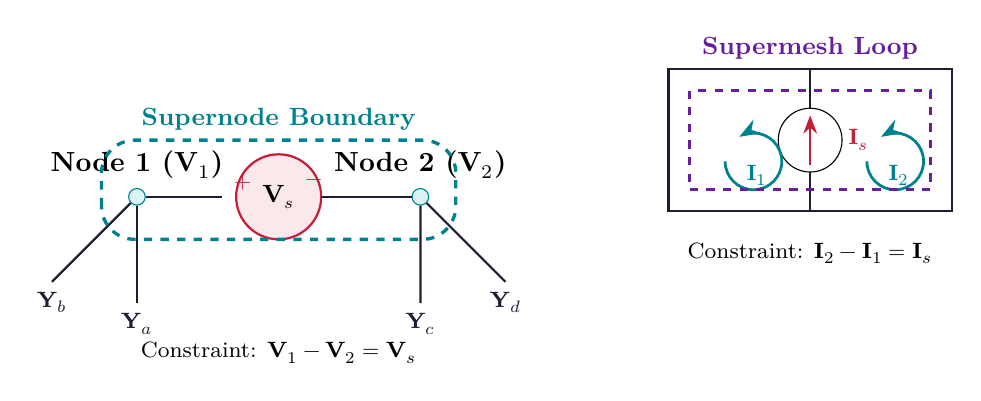
\begin{tikzpicture}[scale=0.9, auto, node distance=2.2cm]
  % Supernode diagram
  \begin{scope}[shift={(0,0)}]
    \node[circnode, label=above:{\textbf{Node 1 ($\mathbf{V}_1$)}}] (n1) at (0,0) {};
    \node[circnode, label=above:{\textbf{Node 2 ($\mathbf{V}_2$)}}] (n2) at (4,0) {};
    
    \draw[line] (n1) -- (1.2,0);
    \draw[draw=myred, fill=hdrred, line width=0.8pt] (2,0) circle (0.6cm) node[font=\small\bfseries] {$\mathbf{V}_s$};
    \node[font=\footnotesize\bfseries, color=myred] at (1.5,0.2) {$+$};
    \node[font=\footnotesize\bfseries, color=myred] at (2.5,0.2) {$-$};
    \draw[line] (2.6,0) -- (n2);
    
    % Branches leaving node 1
    \draw[line] (n1) -- ++(0,-1.5) node[below, font=\footnotesize] {$\mathbf{Y}_a$};
    \draw[line] (n1) -- ++(-1.2,-1.2) node[below, font=\footnotesize] {$\mathbf{Y}_b$};
    
    % Branches leaving node 2
    \draw[line] (n2) -- ++(0,-1.5) node[below, font=\footnotesize] {$\mathbf{Y}_c$};
    \draw[line] (n2) -- ++(1.2,-1.2) node[below, font=\footnotesize] {$\mathbf{Y}_d$};
    
    % Supernode boundary
    \draw[myteal, dashed, line width=1.2pt, rounded corners=12pt] (-0.5,-0.6) rectangle (4.5,0.8);
    \node[color=myteal, font=\small\bfseries] at (2,1.1) {Supernode Boundary};
    \node[font=\footnotesize] at (2,-2.2) {Constraint: $\mathbf{V}_1 - \mathbf{V}_2 = \mathbf{V}_s$};
  \end{scope}

  % Supermesh diagram
  \begin{scope}[shift={(7.5,-0.2)}]
    \draw[line] (0,0) rectangle (4,2);
    \draw[line] (2,0) -- (2,2);
    
    % Current source in shared branch
    \draw[fill=white] (2,1) circle (0.45cm);
    \draw[redarrow] (2,0.65) -- (2,1.35);
    \node[right, font=\footnotesize\bfseries, color=myred] at (2.4,1) {$\mathbf{I}_s$};
    
    % Mesh currents
    \draw[-Stealth, color=myteal, line width=1pt] (0.8,0.7) arc (-180:120:0.4cm) node[midway, left, font=\footnotesize\bfseries] {$\mathbf{I}_1$};
    \draw[-Stealth, color=myteal, line width=1pt] (2.8,0.7) arc (-180:120:0.4cm) node[midway, left, font=\footnotesize\bfseries] {$\mathbf{I}_2$};
    
    % Supermesh boundary
    \draw[mypurple, dashed, line width=1.2pt] (0.3,0.3) -- (3.7,0.3) -- (3.7,1.7) -- (0.3,1.7) -- cycle;
    \node[color=mypurple, font=\small\bfseries] at (2,2.3) {Supermesh Loop};
    \node[font=\footnotesize] at (2,-0.6) {Constraint: $\mathbf{I}_2 - \mathbf{I}_1 = \mathbf{I}_s$};
  \end{scope}
\end{tikzpicture}
\end{tcolorbox}

\subsection{Matrix Mesh (Loop) Impedance Formulation}
For a planar network with $M$ independent meshes, Kirchhoff's Voltage Law (KVL) around clockwise mesh currents yields:
\begin{equation}
  [\mathbf{Z}] \mathbf{I}_m = \mathbf{V}_e
\end{equation}
where:
\begin{equation}
  \begin{bmatrix}
    Z_{11} & Z_{12} & \cdots & Z_{1M} \\
    Z_{21} & Z_{22} & \cdots & Z_{2M} \\
    \vdots & \vdots & \ddots & \vdots \\
    Z_{M1} & Z_{M2} & \cdots & Z_{MM}
  \end{bmatrix}
  \begin{bmatrix}
    \mathbf{I}_1 \\ \mathbf{I}_2 \\ \vdots \\ \mathbf{I}_M
  \end{bmatrix}
  =
  \begin{bmatrix}
    \mathbf{V}_{e1} \\ \mathbf{V}_{e2} \\ \vdots \\ \mathbf{V}_{eM}
  \end{bmatrix}
\end{equation}

\begin{tcolorbox}[formulabox, title={\textbf{Inspection Rules for Mesh Impedance Matrix $[\mathbf{Z}]$}}]
For planar networks with independent voltage sources and passive impedances:
\begin{itemize}[leftmargin=*, itemsep=2pt]
  \item \textbf{Self-Impedance ($Z_{ii}$):} Total sum of all branch impedances forming mesh $i$: $Z_{ii} = \sum Z_{loop\,i}$.
  \item \textbf{Mutual Impedance ($Z_{ij}, i \ne j$):} Negative of the branch impedance common to both mesh $i$ and mesh $j$ when mesh currents flow in opposite directions through the shared branch: $Z_{ij} = -Z_{shared}$.
  \item \textbf{Source Vector ($\mathbf{V}_{ei}$):} Algebraic sum of all independent voltage sources encountered in mesh $i$ clockwise (a potential rise yields positive $\mathbf{V}_e$, a potential drop yields negative $\mathbf{V}_e$).
\end{itemize}
\end{tcolorbox}

\begin{tcolorbox}[defbox, title={\textbf{Supermesh Technique (Current Sources Shared Between Meshes)}}]
When an ideal current source is shared between two adjacent meshes $i$ and $j$:
\begin{enumerate}[leftmargin=*, itemsep=2pt, topsep=1pt]
  \item \textbf{Avoid Shared Branch:} Create a \textbf{supermesh} by conceptually removing the branch containing the current source (leaving an open-circuit path).
  \item \textbf{Apply KVL:} Write one single KVL equation around the combined outer perimeter loop of both meshes.
  \item \textbf{Constraint Equation:} Relate the mesh currents to the current source: $\mathbf{I}_j - \mathbf{I}_i = \mathbf{I}_s$.
\end{enumerate}
\end{tcolorbox}

% ───────────────────────────────────────────────────────────────────────────────
\section{Source Transformation and Network Duality}
% ───────────────────────────────────────────────────────────────────────────────

\subsection{AC Source Transformation}
Any practical AC voltage source consisting of an ideal phasor source $\mathbf{V}_s$ in series with internal impedance $\mathbf{Z}_s$ can be transformed into an equivalent practical AC current source consisting of phasor source $\mathbf{I}_s$ in parallel with internal admittance $\mathbf{Y}_s = 1/\mathbf{Z}_s$:
\begin{equation}
  \mathbf{I}_s = \frac{\mathbf{V}_s}{\mathbf{Z}_s}, \qquad \mathbf{Z}_s = \frac{1}{\mathbf{Y}_s}
\end{equation}
This equivalence holds strictly for all external load terminals at angular frequency $\omega$.

\subsection{Network Duality Principles}
Two networks $N_1$ and $N_2$ are said to be \textbf{dual} to each other if the mesh equations of $N_1$ are mathematically identical in form to the node equations of $N_2$. Duality is an exact topological and algebraic reflection:

\par\vspace{6pt}\noindent
\begingroup
\setlength{\tabcolsep}{6pt}
\setlength{\extrarowheight}{3pt}
\renewcommand{\arraystretch}{1.35}
\begin{tabularx}{\linewidth}{|B{4.5cm}|B{4.5cm}|Y|}
\hline
\multicolumn{1}{|c|}{\textbf{Primary Network Concept}} & \multicolumn{1}{c|}{\textbf{Dual Network Concept}} & \multicolumn{1}{c|}{\textbf{Mathematical Relation}} \\
\hline
Mesh / Loop & Node / Node-Pair & Mesh Current $\mathbf{I}_m \longleftrightarrow$ Node Voltage $\mathbf{V}_n$ \\
\hline
Voltage Law (KVL: $\sum \mathbf{V} = 0$) & Current Law (KCL: $\sum \mathbf{I} = 0$) & Dual equations exchange $V \leftrightarrow I$ \\
\hline
Series Connection & Parallel Connection & $Z = Z_1 + Z_2 \longleftrightarrow Y = Y_1 + Y_2$ \\
\hline
Resistance $R$ ($\Omega$) & Conductance $G$ ($\text{S}$) & $G = R / R_0^2$ (normalized) \\
\hline
Inductance $L$ ($\text{H}$) & Capacitance $C$ ($\text{F}$) & Numerical value: $C = L / R_0^2$ \\
\hline
Voltage Source $\mathbf{V}_s$ & Current Source $\mathbf{I}_s$ & Direction maps clockwise loop $\leftrightarrow$ node entry \\
\hline
Short Circuit ($\mathbf{Z}=0$) & Open Circuit ($\mathbf{Y}=0$) & $\mathbf{V}=0 \longleftrightarrow \mathbf{I}=0$ \\
\hline
\end{tabularx}
\endgroup

\begin{tcolorbox}[tikzbox, title={\textbf{TikZ Schematic: Dual Network Construction on Planar Graphs}}]
\centering
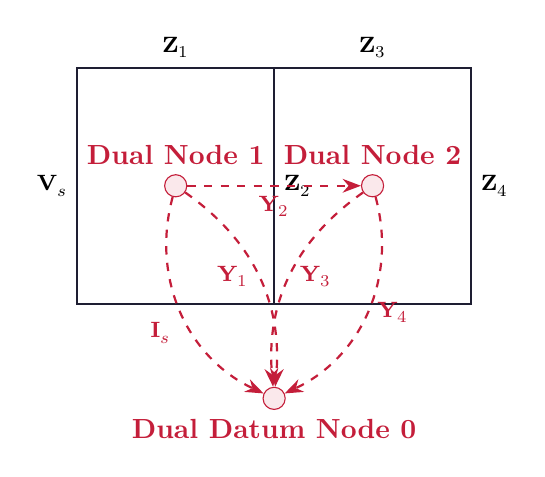
\begin{tikzpicture}[scale=1.0, auto, node distance=2.5cm]
  % Original planar network (Black/Dark lines)
  \draw[line, thick] (0,0) rectangle (5,3);
  \draw[line, thick] (2.5,0) -- (2.5,3);
  
  \node[above, font=\footnotesize\bfseries] at (1.25,3) {$\mathbf{Z}_1$};
  \node[above, font=\footnotesize\bfseries] at (3.75,3) {$\mathbf{Z}_3$};
  \node[left, font=\footnotesize\bfseries] at (0,1.5) {$\mathbf{V}_s$};
  \node[right, font=\footnotesize\bfseries] at (2.5,1.5) {$\mathbf{Z}_2$};
  \node[right, font=\footnotesize\bfseries] at (5,1.5) {$\mathbf{Z}_4$};
  
  % Dual nodes (Red dots in each mesh + 1 outer datum node)
  \node[circle, draw=myred, fill=hdrred, inner sep=2pt, minimum size=8pt, label=above:{\color{myred}\textbf{Dual Node 1}}] (d1) at (1.25,1.5) {};
  \node[circle, draw=myred, fill=hdrred, inner sep=2pt, minimum size=8pt, label=above:{\color{myred}\textbf{Dual Node 2}}] (d2) at (3.75,1.5) {};
  \node[circle, draw=myred, fill=hdrred, inner sep=2pt, minimum size=8pt, label=below:{\color{myred}\textbf{Dual Datum Node 0}}] (d0) at (2.5,-1.2) {};
  
  % Dual branches (Red dashed lines crossing each original branch)
  \draw[redarrow, dashed] (d1) -- (d2) node[midway, below, font=\footnotesize\bfseries] {$\mathbf{Y}_2$};
  \draw[redarrow, dashed] (d1) to[bend left=30] node[left, font=\footnotesize\bfseries] {$\mathbf{Y}_1$} (d0);
  \draw[redarrow, dashed] (d1) to[bend right=40] node[below left, font=\footnotesize\bfseries] {$\mathbf{I}_s$} (d0);
  \draw[redarrow, dashed] (d2) to[bend left=40] node[right, font=\footnotesize\bfseries] {$\mathbf{Y}_4$} (d0);
  \draw[redarrow, dashed] (d2) to[bend right=30] node[right, font=\footnotesize\bfseries] {$\mathbf{Y}_3$} (d0);
\end{tikzpicture}
\end{tcolorbox}

% ───────────────────────────────────────────────────────────────────────────────
\section{Network Theorems as Applied to AC Circuits}
% ───────────────────────────────────────────────────────────────────────────────

\subsection{Superposition Theorem (AC Form)}

\begin{tcolorbox}[defbox, title={\textbf{Superposition Theorem Statement}}]
In any linear, bilateral AC electrical network containing multiple independent sources operating at identical or differing frequencies, the steady-state phasor response (current or voltage) in any branch equals the algebraic sum of the individual phasor responses produced by each independent source acting alone, with all other independent sources set to zero:
\begin{itemize}[leftmargin=*, itemsep=2pt, topsep=1pt]
  \item Independent voltage sources are replaced by short circuits ($\mathbf{V}_s = 0$).
  \item Independent current sources are replaced by open circuits ($\mathbf{I}_s = 0$).
  \item Dependent sources remain untouched and active throughout the procedure.
\end{itemize}
\end{tcolorbox}

\begin{tcolorbox}[examplebox, title={\textbf{Critical Exam Caveat: Superposition with Differing Frequencies and AC Power}}]
\textbf{1. Multi-Frequency Superposition:} If sources operate at distinct angular frequencies ($\omega_1 \ne \omega_2$), phasors \textbf{cannot} be added algebraically in the frequency domain because they exist on different complex bases. Responses must be calculated individually as time functions and summed in the time domain:
\begin{equation}
  v(t) = v_1(t) + v_2(t) = V_{m1} \cos(\omega_1 t + \phi_1) + V_{m2} \cos(\omega_2 t + \phi_2)
\end{equation}
\textbf{2. Average Power is Non-Linear:} Superposition does \textbf{not} hold for power ($P \ne P_1 + P_2$) when sources share the same frequency, because $P \propto I^2 = (I_1 + I_2)^2 = I_1^2 + I_2^2 + 2 I_1 I_2$. Only when sources have orthogonal frequencies ($\omega_1 \ne \omega_2$) does the cross-product average to zero, allowing:
\begin{equation}
  P_{\text{avg}} = P_1 + P_2 \qquad (\text{strictly for } \omega_1 \ne \omega_2)
\end{equation}
\end{tcolorbox}

\subsection{Thevenin's and Norton's Theorems (AC Form)}

\begin{tcolorbox}[defbox, title={\textbf{Thevenin's and Norton's AC Theorems}}]
\textbf{Thevenin's Theorem:} Any linear, bilateral, active two-terminal AC network can be replaced at its external load terminals ($A$-$B$) by an equivalent circuit consisting of an open-circuit phasor voltage source $\mathbf{V}_{th}$ connected in series with an internal equivalent impedance $\mathbf{Z}_{th}$.

\textbf{Norton's Theorem:} The same two-terminal AC network can alternatively be replaced by an ideal short-circuit phasor current source $\mathbf{I}_N$ connected in parallel with an internal equivalent admittance $\mathbf{Y}_N = 1/\mathbf{Z}_{th}$.
\end{tcolorbox}

\begin{tcolorbox}[formulabox, title={\textbf{Analytical Formulation and Evaluation of $\mathbf{V}_{th}, \mathbf{I}_N$ and $\mathbf{Z}_{th}$}}]
\begin{itemize}[leftmargin=*, itemsep=2pt]
  \item \textbf{Open-Circuit Voltage ($\mathbf{V}_{th}$):} $\mathbf{V}_{th} = \mathbf{V}_{oc} = \mathbf{V}_A - \mathbf{V}_B$ across open terminals $A$-$B$.
  \item \textbf{Short-Circuit Current ($\mathbf{I}_N$):} $\mathbf{I}_N = \mathbf{I}_{sc}$ flowing from terminal $A$ to $B$ when short-circuited.
  \item \textbf{Source Inter-relation:} $\mathbf{V}_{th} = \mathbf{I}_N \cdot \mathbf{Z}_{th}$.
  \item \textbf{Evaluation of $\mathbf{Z}_{th}$ (Networks with Dependent Sources):} Deactivate all independent sources. Apply an external test source $\mathbf{V}_{\text{test}}$ across terminals $A$-$B$ and compute resulting input current $\mathbf{I}_{\text{test}}$:
  \begin{equation}
    \mathbf{Z}_{th} = \frac{\mathbf{V}_{\text{test}}}{\mathbf{I}_{\text{test}}} = \frac{\mathbf{V}_{oc}}{\mathbf{I}_{sc}}
  \end{equation}
\end{itemize}
\end{tcolorbox}

\subsection{Maximum Power Transfer Theorem in AC Circuits}
Let a linear AC source be represented by its Thevenin equivalent ($\mathbf{V}_{th}, \mathbf{Z}_{th} = R_{th} + jX_{th}$) driving a complex load impedance $\mathbf{Z}_L = R_L + jX_L$.

\begin{tcolorbox}[formulabox, title={\textbf{Derivation: Condition for Maximum Average Power Transfer}}]
The phasor current through the load is:
\begin{equation}
  \mathbf{I}_L = \frac{\mathbf{V}_{th}}{\mathbf{Z}_{th} + \mathbf{Z}_L} = \frac{\mathbf{V}_{th}}{(R_{th} + R_L) + j(X_{th} + X_L)}
\end{equation}
The magnitude of the load current squared is:
\begin{equation}
  |\mathbf{I}_L|^2 = \frac{|\mathbf{V}_{th}|^2}{(R_{th} + R_L)^2 + (X_{th} + X_L)^2}
\end{equation}
The real average power dissipated in load resistance $R_L$ is:
\begin{equation}
  P_L = |\mathbf{I}_L|^2 R_L = \frac{|\mathbf{V}_{th}|^2 R_L}{(R_{th} + R_L)^2 + (X_{th} + X_L)^2}
\end{equation}
\textbf{Step 1: Optimization with respect to $X_L$:}
To maximize $P_L$, the denominator must be minimized. Setting $\frac{\partial P_L}{\partial X_L} = 0$:
\begin{equation}
  X_L + X_{th} = 0 \implies \mathbf{X}_L = -\mathbf{X}_{th}
\end{equation}
The load reactance must cancel the source reactance (conjugate match condition).

\textbf{Step 2: Optimization with respect to $R_L$:}
With $X_L = -X_{th}$, $P_L = \frac{|\mathbf{V}_{th}|^2 R_L}{(R_{th} + R_L)^2}$. Setting $\frac{dP_L}{dR_L} = 0$:
\begin{equation}
  \frac{d}{dR_L}\left[ \frac{R_L}{(R_{th} + R_L)^2} \right] = \frac{(R_{th} + R_L)^2 - 2R_L(R_{th} + R_L)}{(R_{th} + R_L)^4} = 0 \implies \mathbf{R}_L = \mathbf{R}_{th}
\end{equation}
Combining both conditions yields the \textbf{Complex Conjugate Match}:
\begin{equation}
  \mathbf{Z}_L = R_{th} - jX_{th} = \mathbf{Z}_{th}^*
\end{equation}
The corresponding maximum average power delivered to the load is:
\begin{equation}
  P_{\max} = \frac{|\mathbf{V}_{th}|^2 R_{th}}{(2R_{th})^2} = \frac{|\mathbf{V}_{th}|^2}{4 R_{th}}
\end{equation}
\end{tcolorbox}

\subsubsection{Constrained Load Cases}
\begin{enumerate}[leftmargin=*, itemsep=2pt]
  \item \textbf{Load Phase Angle Fixed ($\mathbf{Z}_L = |Z_L|\angle \theta_L$ with variable magnitude):}
  \begin{equation}
    |Z_L| = |Z_{th}| = \sqrt{R_{th}^2 + X_{th}^2}
  \end{equation}
  \item \textbf{Purely Resistive Load ($X_L = 0, R_L$ variable):}
  \begin{equation}
    R_L = |\mathbf{Z}_{th}| = \sqrt{R_{th}^2 + X_{th}^2}
  \end{equation}
  \item \textbf{Fixed Reactance $X_L$ with Variable Resistance $R_L$:}
  \begin{equation}
    R_L = \sqrt{R_{th}^2 + (X_{th} + X_L)^2}
  \end{equation}
\end{enumerate}

\subsection{Reciprocity Theorem}

\begin{tcolorbox}[defbox, title={\textbf{Reciprocity Theorem in AC Networks}}]
In any linear, bilateral, passive, time-invariant AC network, if an ideal voltage source $\mathbf{V}_1$ applied in branch 1 produces a current $\mathbf{I}_2$ in branch 2, then the same voltage source transferred to branch 2 will produce identical current $\mathbf{I}_1 = \mathbf{I}_2$ in branch 1:
\begin{equation}
  \mathbf{Z}_{12} = \frac{\mathbf{V}_1}{\mathbf{I}_2} = \frac{\mathbf{V}_2}{\mathbf{I}_1} = \mathbf{Z}_{21}
\end{equation}
The transfer impedance is completely symmetrical ($\mathbf{Z}_{12} = \mathbf{Z}_{21}$).
\end{tcolorbox}
\par\vspace{4pt}\noindent
\textbf{Restrictions:} The network must contain no dependent sources, no unilateral devices (like diodes), and only a single source must be active.

\subsection{Compensation (Substitution) Theorem}
If the impedance of a branch carrying steady-state phasor current $\mathbf{I}$ changes by an increment $\Delta\mathbf{Z}$ (from $\mathbf{Z}$ to $\mathbf{Z} + \Delta\mathbf{Z}$), the incremental change in currents and voltages throughout all other branches in the network can be calculated by replacing the altered impedance with a virtual compensation voltage source $\mathbf{V}_c$:
\begin{equation}
  \mathbf{V}_c = \mathbf{I}' \Delta\mathbf{Z} \approx \mathbf{I} \Delta\mathbf{Z}
\end{equation}
directed in opposition to the original current $\mathbf{I}$, while deactivating all original independent sources.

\subsection{Tellegen's Theorem}

\begin{tcolorbox}[defbox, title={\textbf{Tellegen's Theorem}}]
For any lumped electrical network containing $b$ branches and $n$ nodes, whose branch voltages $v_k(t)$ satisfy KVL and branch currents $i_k(t)$ satisfy KCL under associated reference directions:
\begin{equation}
  \sum_{k=1}^b v_k(t) i_k(t) = 0 \qquad \text{at every instant } t
\end{equation}
In the frequency domain for AC steady-state sinusoidal circuits:
\begin{equation}
  \sum_{k=1}^b \mathbf{V}_k \mathbf{I}_k^* = 0 \implies \sum_{k=1}^b P_k + j \sum_{k=1}^b Q_k = 0
\end{equation}
The sum of complex powers delivered to all branches is identically zero (conservation of both active power $P$ and reactive power $Q$).
\end{tcolorbox}

\textbf{Remarkable Scope:} Tellegen's theorem is completely independent of the nature of the network components. It holds whether elements are linear, non-linear, passive, active, time-varying, or time-invariant; it relies solely on the topological graph properties governed by KVL and KCL.

\newpage
% ===============================================================================
% MANDATORY QUICK REVISION PAGE
% ===============================================================================
\begin{center}
  {\large\bfseries\color{myred} Quick Revision --- Module 1}\\[3pt]
  {\small\color{mydark} Mesh, Nodal Analysis and AC Network Theorems $|$ EC304}
\end{center}
\noindent{\color{myred}\rule{\linewidth}{1.2pt}}
\vspace{4pt}

\begin{tcolorbox}[formulabox, title={\textbf{Key Formulas and Network Relations at a Glance}}]
\renewcommand{\arraystretch}{1.35}
\begin{tabularx}{\linewidth}{B{5.0cm} X}
Inductive Reactance & $X_L = \omega L, \quad \mathbf{Z}_L = j\omega L = \omega L \angle 90^\circ$ \\[4pt]
Capacitive Reactance & $X_C = \frac{1}{\omega C}, \quad \mathbf{Z}_C = \frac{-j}{\omega C} = \frac{1}{\omega C} \angle -90^\circ$ \\[4pt]
Nodal Admittance Matrix & $[\mathbf{Y}]\mathbf{V}_n = \mathbf{I}_s, \quad Y_{ii} = \sum y_{branch}, \quad Y_{ij} = -y_{ij}$ \\[4pt]
Mesh Impedance Matrix & $[\mathbf{Z}]\mathbf{I}_m = \mathbf{V}_e, \quad Z_{ii} = \sum Z_{loop}, \quad Z_{ij} = -Z_{shared}$ \\[4pt]
Source Transformation & $\mathbf{I}_s = \mathbf{V}_s / \mathbf{Z}_s, \quad \mathbf{Z}_s = 1 / \mathbf{Y}_s$ \\[4pt]
Maximum Power Condition (AC) & $\mathbf{Z}_L = \mathbf{Z}_{th}^* = R_{th} - jX_{th}$ \\[4pt]
Maximum Power Formula & $P_{\max} = \frac{|\mathbf{V}_{th}|^2}{4 R_{th}} \quad (\text{W})$ \\[4pt]
Resistive Load Max Power & $R_L = |\mathbf{Z}_{th}| = \sqrt{R_{th}^2 + X_{th}^2}$ \\[4pt]
Reciprocity Transfer Symmetry & $\mathbf{Z}_{12} = \frac{\mathbf{V}_1}{\mathbf{I}_2} = \frac{\mathbf{V}_2}{\mathbf{I}_1} = \mathbf{Z}_{21}$ \\[4pt]
Tellegen's Complex Conservation & $\sum_{k=1}^b \mathbf{V}_k \mathbf{I}_k^* = 0 \iff \sum P_k = 0 \text{ and } \sum Q_k = 0$ \\[4pt]
\end{tabularx}
\end{tcolorbox}

\begin{tcolorbox}[defbox, title={\textbf{One-Line Definitions}}]
\begin{itemize}[leftmargin=*, itemsep=2pt, topsep=0pt]
  \item \textbf{Phasor:} A complex representation of a sinusoidal voltage or current containing amplitude and phase angle.
  \item \textbf{Impedance ($\mathbf{Z}$):} Total opposition offered by a network element to sinusoidal alternating current, measured in ohms.
  \item \textbf{Admittance ($\mathbf{Y}$):} The measure of ease with which an AC circuit allows current to flow, defined as $1/\mathbf{Z}$.
  \item \textbf{Supernode:} A generalized node created by enclosing a voltage source connected between two non-reference nodes.
  \item \textbf{Supermesh:} A combined loop formed by avoiding a branch containing an ideal current source shared between two meshes.
  \item \textbf{Dual Networks:} Two networks whose loop equations in one are structurally and mathematically identical to the node equations in the other.
  \item \textbf{Thevenin Equivalent:} An AC circuit reduction consisting of an open-circuit voltage $\mathbf{V}_{th}$ in series with $\mathbf{Z}_{th}$.
  \item \textbf{Norton Equivalent:} An AC circuit reduction consisting of a short-circuit current $\mathbf{I}_N$ in parallel with $\mathbf{Z}_{th}$.
  \item \textbf{Conjugate Match:} Setting load impedance equal to the complex conjugate of source impedance for maximum power transfer.
  \item \textbf{Tellegen's Theorem:} A topological theorem stating that the sum of power delivered over all branches in any lumped network is zero.
\end{itemize}
\end{tcolorbox}

\begin{tcolorbox}[exambox, title={\textbf{Frequently Asked / Viva Questions}}]
\begin{enumerate}[topsep=0pt, label=\textbf{Q\arabic*.}, itemsep=5pt]
  \item \Q{State the condition for maximum power transfer in an AC circuit with complex source and load impedances.}
  Maximum active power transfer occurs when the load impedance is the complex conjugate of the Thevenin impedance: $\mathbf{Z}_L = \mathbf{Z}_{th}^* = R_{th} - jX_{th}$. Under this condition, reactive power cancels out, and $P_{\max} = \frac{|\mathbf{V}_{th}|^2}{4 R_{th}}$.

  \item \Q{Why can the superposition theorem not be directly applied to calculate total AC power?}
  Because power is a non-linear quadratic function of voltage and current ($P = I^2 R$). The square of a sum contains cross-product terms: $(I_1 + I_2)^2 = I_1^2 + I_2^2 + 2 I_1 I_2 \ne I_1^2 + I_2^2$. Therefore, currents or voltages must be superposed first, and power calculated subsequently from the net total.

  \item \Q{How do you evaluate Thevenin impedance $\mathbf{Z}_{th}$ in a circuit containing dependent sources?}
  Deactivate all independent sources (short voltage sources, open current sources). Connect a fictitious test source $\mathbf{V}_{\text{test}}$ across the open terminals, determine the resulting current $\mathbf{I}_{\text{test}}$ supplied by the test source, and compute $\mathbf{Z}_{th} = \mathbf{V}_{\text{test}} / \mathbf{I}_{\text{test}}$.

  \item \Q{What are the fundamental requirements for the Reciprocity theorem to hold in a network?}
  The network must be linear, passive, time-invariant, bilateral, and contain no dependent sources or non-linear elements. Only a single excitation source must be active at a time.

  \item \Q{What is the physical meaning of Tellegen's theorem in an AC circuit?}
  It proves that in any lumped network, the sum of all instantaneous branch powers equals zero. In AC circuits, this implies the simultaneous conservation of both active real power ($\sum P_k = 0$) and reactive imaginary power ($\sum Q_k = 0$).

  \item \Q{When is a supernode required in nodal analysis?}
  When an ideal voltage source (independent or dependent) is connected directly between two non-reference nodes without any series impedance, making the branch current indeterminate from node voltages alone.

  \item \Q{Explain the concept of duality in electrical networks.}
  Two planar networks are duals if the KVL loop equations of one match the KCL node equations of the other. Series branches map to parallel branches, meshes map to nodes, inductors map to capacitors, and voltage sources map to current sources.

  \item \Q{If the load is purely resistive ($X_L = 0$), what is the condition for maximum power transfer from an AC source?}
  The load resistance must equal the magnitude of the source Thevenin impedance: $R_L = |\mathbf{Z}_{th}| = \sqrt{R_{th}^2 + X_{th}^2}$.

  \item \Q{Can Tellegen's theorem be applied to non-linear and time-varying circuits?}
  Yes. Tellegen's theorem depends strictly on Kirchhoff's laws (KVL and KCL), which stem solely from topology (conservation of energy and charge). It holds irrespective of whether elements are linear, non-linear, active, passive, or time-varying.

  \item \Q{What is the difference between Mesh Analysis and Loop Analysis?}
  A mesh is a loop that does not contain any other loops within it (applicable strictly to planar circuits). Loop analysis can be applied to arbitrary closed paths and non-planar networks using fundamental loop sets.
\end{enumerate}
\end{tcolorbox}

\begin{tcolorbox}[tikzbox, title={\textbf{Summary Matrix: Comprehensive Comparison of AC Network Theorems}}]
\par\vspace{4pt}\noindent
\begingroup
\setlength{\tabcolsep}{4.5pt}
\setlength{\extrarowheight}{3pt}
\renewcommand{\arraystretch}{1.35}
\begin{tabularx}{\linewidth}{|B{3.2cm}|B{3.5cm}|Y|}
\hline
\multicolumn{1}{|c|}{\textbf{Theorem}} & \multicolumn{1}{c|}{\textbf{Primary Condition}} & \multicolumn{1}{c|}{\textbf{Practical Applications and Limitations}} \\
\hline
Superposition & Linear, bilateral elements & Multi-frequency circuits; invalid for power calculations. \\
\hline
Thevenin's & Linear active two-terminal & Simplifies terminal analysis; $\mathbf{Z}_{th}$ needs test source if dependent sources exist. \\
\hline
Norton's & Dual of Thevenin's theorem & Current-driven systems; relates via $\mathbf{V}_{th} = \mathbf{I}_N \mathbf{Z}_{th}$. \\
\hline
Maximum Power Transfer & Source $\mathbf{Z}_{th}$ fixed, load adjustable & Conjugate match $\mathbf{Z}_L = \mathbf{Z}_{th}^*$; efficiency is strictly $50\%$. \\
\hline
Reciprocity & Linear, bilateral, passive, no dependent sources & Symmetrical transfer impedance; useful in antennas and filters. \\
\hline
Tellegen's & Any lumped network obeying KVL \& KCL & Holds for linear/non-linear, active/passive; confirms energy conservation. \\
\hline
\end{tabularx}
\endgroup
\end{tcolorbox}


% -- Module 2 -----------------------------------------------------------------
\modulestart{2}{Fourier Series Analysis in Electrical Networks}

\section{Fourier Series Analysis in Electrical Networks}
% ───────────────────────────────────────────────────────────────────────────────

\begin{tcolorbox}[defbox, title={\textbf{Definition: Trigonometric and Exponential Fourier Series}}]
Any physically realizable periodic electrical signal $f(t) = f(t + T)$ with fundamental period $T$ and fundamental angular frequency $\omega_0 = 2\pi/T$ satisfying the Dirichlet conditions can be decomposed into an infinite sum of harmonically related sinusoids:
\begin{enumerate}[leftmargin=*, itemsep=2pt, topsep=1pt]
  \item \textbf{Trigonometric Fourier Series (TFS):}
  \begin{equation}
    f(t) = a_0 + \sum_{n=1}^\infty \left[ a_n \cos(n\omega_0 t) + b_n \sin(n\omega_0 t) \right]
  \end{equation}
  where the Fourier coefficients are defined over any arbitrary period $t_0$ to $t_0 + T$:
  \begin{equation}
    a_0 = \frac{1}{T} \int_{t_0}^{t_0+T} f(t)\,dt, \qquad a_n = \frac{2}{T} \int_{t_0}^{t_0+T} f(t) \cos(n\omega_0 t)\,dt
  \end{equation}
  \begin{equation}
    b_n = \frac{2}{T} \int_{t_0}^{t_0+T} f(t) \sin(n\omega_0 t)\,dt
  \end{equation}
  \item \textbf{Compact (Harmonic) Trigonometric Form:}
  \begin{equation}
    f(t) = c_0 + \sum_{n=1}^\infty c_n \cos(n\omega_0 t - \theta_n), \quad c_0 = a_0, \quad c_n = \sqrt{a_n^2 + b_n^2}, \quad \theta_n = \tan^{-1}\left(\frac{b_n}{a_n}\right)
  \end{equation}
  \item \textbf{Exponential Fourier Series (EFS):}
  \begin{equation}
    f(t) = \sum_{n=-\infty}^\infty C_n e^{j n \omega_0 t}, \qquad C_n = \frac{1}{T} \int_{t_0}^{t_0+T} f(t) e^{-j n \omega_0 t} dt
  \end{equation}
\end{enumerate}
\end{tcolorbox}

\subsection{Inter-relationship Between Coefficients}
The complex exponential and real trigonometric coefficients relate directly via Euler's identities:
\begin{equation}
  C_0 = a_0, \qquad C_n = \frac{a_n - jb_n}{2} = \frac{c_n}{2} e^{-j\theta_n}, \qquad C_{-n} = C_n^* = \frac{a_n + jb_n}{2}
\end{equation}
Conversely:
\begin{equation}
  a_n = C_n + C_{-n} = 2 \text{Re}\{C_n\}, \qquad b_n = j(C_n - C_{-n}) = -2 \text{Im}\{C_n\}
\end{equation}

\subsection{Waveform Symmetry and Harmonic Content}
Exploiting waveform symmetry simplifies Fourier integration and provides immediate diagnostic criteria for harmonic absence:

\par\vspace{6pt}\noindent
\begingroup
\setlength{\tabcolsep}{4.5pt}
\setlength{\extrarowheight}{2.5pt}
\renewcommand{\arraystretch}{1.30}
\begin{tabularx}{\linewidth}{|B{2.6cm}|B{3.2cm}|B{3.2cm}|Y|}
\hline
\textbf{Symmetry Type} & \textbf{Condition} & \textbf{Zero Coefficients} & \textbf{Surviving Harmonics} \\
\hline
Even Symmetry & $f(-t) = f(t)$ & $b_n = 0 \quad \forall n$ & DC component and cosine harmonics only. \\
\hline
Odd Symmetry & $f(-t) = -f(t)$ & $a_0 = 0, \quad a_n = 0 \quad \forall n$ & Sine harmonics only (strictly no DC). \\
\hline
Half-Wave (HWS) & $f(t \pm \frac{T}{2}) = -f(t)$ & $a_0 = 0, \; a_{2k} = b_{2k} = 0$ & Strictly odd harmonics only ($n = 1, 3, 5, \dots$). \\
\hline
Even Quarter-Wave & HWS $+$ Even & $a_0 = 0, \; b_n = 0 \quad \forall n$ & Odd cosine harmonics only ($a_{2k+1}$). \\
\hline
Odd Quarter-Wave & HWS $+$ Odd & $a_0 = 0, \; a_n = 0 \quad \forall n$ & Odd sine harmonics only ($b_{2k+1}$). \\
\hline
\end{tabularx}
\endgroup

\begin{tcolorbox}[tikzbox, title={\textbf{TikZ Illustration: Discrete Line Spectra of a Periodic Signal}}]
\centering
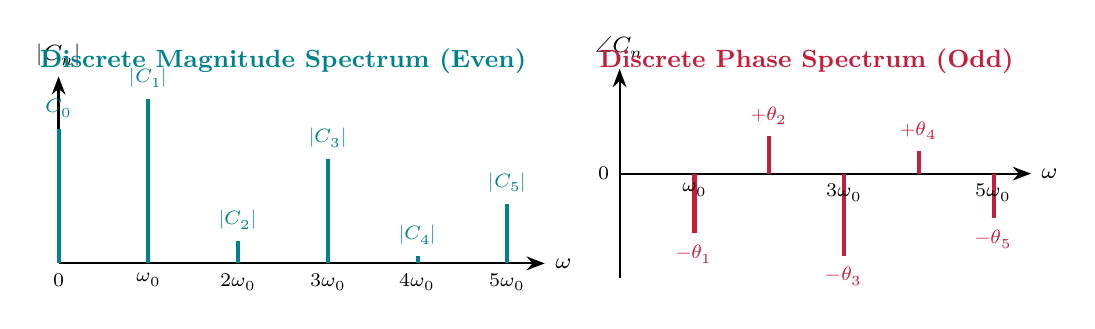
\begin{tikzpicture}[scale=0.95, auto]
  % Magnitude Spectrum
  \draw[-Stealth, thick] (0,0) -- (6.5,0) node[right, font=\footnotesize] {$\omega$};
  \draw[-Stealth, thick] (0,0) -- (0,2.5) node[above, font=\footnotesize] {$|C_n|$};
  \node[below, font=\scriptsize] at (0,0) {$0$};
  
  \draw[line width=1.5pt, color=myteal] (0,0) -- (0,1.8) node[above, font=\scriptsize\bfseries] {$C_0$};
  \draw[line width=1.5pt, color=myteal] (1.2,0) -- (1.2,2.2) node[above, font=\scriptsize\bfseries] {$|C_1|$};
  \draw[line width=1.5pt, color=myteal] (2.4,0) -- (2.4,0.3) node[above, font=\scriptsize\bfseries] {$|C_2|$};
  \draw[line width=1.5pt, color=myteal] (3.6,0) -- (3.6,1.4) node[above, font=\scriptsize\bfseries] {$|C_3|$};
  \draw[line width=1.5pt, color=myteal] (4.8,0) -- (4.8,0.1) node[above, font=\scriptsize\bfseries] {$|C_4|$};
  \draw[line width=1.5pt, color=myteal] (6.0,0) -- (6.0,0.8) node[above, font=\scriptsize\bfseries] {$|C_5|$};
  
  \node[below, font=\scriptsize] at (1.2,0) {$\omega_0$};
  \node[below, font=\scriptsize] at (2.4,0) {$2\omega_0$};
  \node[below, font=\scriptsize] at (3.6,0) {$3\omega_0$};
  \node[below, font=\scriptsize] at (4.8,0) {$4\omega_0$};
  \node[below, font=\scriptsize] at (6.0,0) {$5\omega_0$};
  \node[font=\small\bfseries, color=myteal] at (3.0, 2.7) {Discrete Magnitude Spectrum (Even)};

  % Phase Spectrum (Shifted)
  \begin{scope}[shift={(7.5,1.2)}]
    \draw[-Stealth, thick] (0,0) -- (5.5,0) node[right, font=\footnotesize] {$\omega$};
    \draw[-Stealth, thick] (0,-1.4) -- (0,1.4) node[above, font=\footnotesize] {$\angle C_n$};
    \node[left, font=\scriptsize] at (0,0) {$0$};
    
    \draw[line width=1.5pt, color=myred] (1.0,0) -- (1.0,-0.8) node[below, font=\scriptsize\bfseries] {$-\theta_1$};
    \draw[line width=1.5pt, color=myred] (2.0,0) -- (2.0,0.5) node[above, font=\scriptsize\bfseries] {$+\theta_2$};
    \draw[line width=1.5pt, color=myred] (3.0,0) -- (3.0,-1.1) node[below, font=\scriptsize\bfseries] {$-\theta_3$};
    \draw[line width=1.5pt, color=myred] (4.0,0) -- (4.0,0.3) node[above, font=\scriptsize\bfseries] {$+\theta_4$};
    \draw[line width=1.5pt, color=myred] (5.0,0) -- (5.0,-0.6) node[below, font=\scriptsize\bfseries] {$-\theta_5$};
    
    \node[below, font=\scriptsize] at (1.0,0) {$\omega_0$};
    \node[below, font=\scriptsize] at (3.0,0) {$3\omega_0$};
    \node[below, font=\scriptsize] at (5.0,0) {$5\omega_0$};
    \node[font=\small\bfseries, color=myred] at (2.5, 1.5) {Discrete Phase Spectrum (Odd)};
  \end{scope}
\end{tikzpicture}
\end{tcolorbox}

% ───────────────────────────────────────────────────────────────────────────────
\section{Network Response to Non-Sinusoidal Periodic Inputs}
% ───────────────────────────────────────────────────────────────────────────────

\subsection{Harmonic Superposition Method}
When a linear time-invariant circuit is excited by a non-sinusoidal periodic voltage source:
\begin{equation}
  v(t) = V_0 + \sum_{n=1}^\infty V_{mn} \cos(n\omega_0 t + \theta_{vn})
\end{equation}
the steady-state current response is calculated by applying the \textbf{Superposition Principle} to each harmonic component independently.

\begin{tcolorbox}[formulabox, title={\textbf{Systematic Harmonic Solution Procedure}}]
\begin{enumerate}[leftmargin=*, itemsep=2pt, topsep=1pt]
  \item \textbf{DC Analysis ($n=0$):} Replace inductors with short circuits ($\mathbf{Z}_L = 0$) and capacitors with open circuits ($\mathbf{Z}_C = \infty$). Compute DC current:
  \begin{equation}
    I_0 = \frac{V_0}{R_{\text{eq}}}
  \end{equation}
  \item \textbf{$n$-th Harmonic Impedance:} Evaluate network input impedance at harmonic frequency $\omega_n = n\omega_0$:
  \begin{equation}
    \mathbf{Z}(j n \omega_0) = R_n + j X_n = |\mathbf{Z}_n| e^{j \phi_n} = |\mathbf{Z}_n| \angle \phi_n
  \end{equation}
  where inductive reactance scales directly ($X_{Ln} = n\omega_0 L$) and capacitive reactance scales inversely ($X_{Cn} = \frac{1}{n\omega_0 C}$).
  \item \textbf{$n$-th Harmonic Current Phasor:}
  \begin{equation}
    \mathbf{I}_{mn} = \frac{\mathbf{V}_{mn} \angle \theta_{vn}}{|\mathbf{Z}_n| \angle \phi_n} = \frac{V_{mn}}{|\mathbf{Z}_n|} \angle (\theta_{vn} - \phi_n) = I_{mn} \angle \theta_{in}
  \end{equation}
  \item \textbf{Total Time-Domain Current Synthesis:}
  \begin{equation}
    i(t) = I_0 + \sum_{n=1}^\infty I_{mn} \cos(n\omega_0 t + \theta_{vn} - \phi_n)
  \end{equation}
\end{enumerate}
\end{tcolorbox}

\subsection{Effective (RMS) Values and Average Power}

\begin{tcolorbox}[formulabox, title={\textbf{Formulas for RMS Values and Non-Sinusoidal Power}}]
\begin{itemize}[leftmargin=*, itemsep=3pt]
  \item \textbf{True RMS (Effective) Voltage and Current:}
  \begin{equation}
    V_{\text{rms}} = \sqrt{\frac{1}{T}\int_0^T v^2(t) dt} = \sqrt{V_0^2 + \sum_{n=1}^\infty \frac{V_{mn}^2}{2}} = \sqrt{V_0^2 + \sum_{n=1}^\infty V_{n,\text{rms}}^2}
  \end{equation}
  \begin{equation}
    I_{\text{rms}} = \sqrt{I_0^2 + \sum_{n=1}^\infty I_{n,\text{rms}}^2}
  \end{equation}
  \item \textbf{Total Average Active Power ($P$):} By orthogonality of distinct sinusoids over fundamental period $T$, all cross-harmonic terms integrate to zero:
  \begin{equation}
    P = \frac{1}{T}\int_0^T v(t) i(t) dt = V_0 I_0 + \sum_{n=1}^\infty V_{n,\text{rms}} I_{n,\text{rms}} \cos(\phi_n)
  \end{equation}
  \item \textbf{Apparent Power ($S$), Reactive Power ($Q$) and Distortion Power ($D$):}
  \begin{equation}
    S = V_{\text{rms}} I_{\text{rms}}, \qquad Q = \sum_{n=1}^\infty V_{n,\text{rms}} I_{n,\text{rms}} \sin(\phi_n), \qquad D = \sqrt{S^2 - P^2 - Q^2}
  \end{equation}
  \item \textbf{True Power Factor and Distortion Factor:}
  \begin{equation}
    \text{PF} = \frac{P}{S} = \frac{I_{1,\text{rms}}}{I_{\text{rms}}} \cdot \cos\phi_1 = (\text{Distortion Factor}) \times (\text{Displacement Factor})
  \end{equation}
  \item \textbf{Total Harmonic Distortion (THD):}
  \begin{equation}
    \text{THD}_I = \frac{\sqrt{\sum_{n=2}^\infty I_{n,\text{rms}}^2}}{I_{1,\text{rms}}} = \sqrt{\left(\frac{I_{\text{rms}}}{I_{1,\text{rms}}}\right)^2 - 1}
  \end{equation}
\end{itemize}
\end{tcolorbox}

% ───────────────────────────────────────────────────────────────────────────────
\section{The Continuous Spectrum via Fourier Transform}
% ───────────────────────────────────────────────────────────────────────────────

\begin{tcolorbox}[defbox, title={\textbf{Continuous Fourier Transform Pair}}]
As period $T \to \infty$, discrete spectral lines merge into a continuous density spectrum:
\begin{equation}
  X(j\omega) = \mathcal{F}\{x(t)\} = \int_{-\infty}^\infty x(t) e^{-j\omega t} dt
\end{equation}
\begin{equation}
  x(t) = \mathcal{F}^{-1}\{X(j\omega)\} = \frac{1}{2\pi} \int_{-\infty}^\infty X(j\omega) e^{j\omega t} d\omega
\end{equation}
\end{tcolorbox}
\par\vspace{4pt}\noindent
The \textbf{Energy Spectral Density} is $\mathcal{E}(\omega) = |X(j\omega)|^2$. Total signal energy is conserved under the transformation via \textbf{Parseval's Energy Theorem}:
\begin{equation}
  W = \int_{-\infty}^\infty |x(t)|^2 dt = \frac{1}{2\pi} \int_{-\infty}^\infty |X(j\omega)|^2 d\omega
\end{equation}

% ───────────────────────────────────────────────────────────────────────────────
\section{Three-Phase Unbalanced Circuits and Symmetrical Components}
% ───────────────────────────────────────────────────────────────────────────────

\subsection{Symmetrical Components Transformation (Fortescue's Theorem)}
In an unbalanced three-phase system, the three unsymmetrical phasor voltages or currents can be decomposed into three balanced symmetrical components:

\begin{tcolorbox}[defbox, title={\textbf{Fortescue's Theorem and the Complex Operator $a$}}]
Any set of three unbalanced phasors $\mathbf{V}_a, \mathbf{V}_b, \mathbf{V}_c$ can be uniquely expressed as the sum of three balanced symmetrical sets:
\begin{enumerate}[leftmargin=*, itemsep=2pt, topsep=1pt]
  \item \textbf{Positive-Sequence ($\mathbf{V}_{a1}, \mathbf{V}_{b1}, \mathbf{V}_{c1}$):} Equal magnitudes, $120^\circ$ phase separation, same phase sequence ($a$-$b$-$c$) as original.
  \item \textbf{Negative-Sequence ($\mathbf{V}_{a2}, \mathbf{V}_{b2}, \mathbf{V}_{c2}$):} Equal magnitudes, $120^\circ$ phase separation, reversed phase sequence ($a$-$c$-$b$).
  \item \textbf{Zero-Sequence ($\mathbf{V}_{a0}, \mathbf{V}_{b0}, \mathbf{V}_{c0}$):} Equal magnitudes and identical phase angles (in-phase).
\end{enumerate}
Defining the complex phase-shift operator $a = e^{j 120^\circ} = -\frac{1}{2} + j\frac{\sqrt{3}}{2}$:
\begin{equation}
  a^2 = e^{j 240^\circ} = -\frac{1}{2} - j\frac{\sqrt{3}}{2}, \qquad a^3 = 1, \qquad 1 + a + a^2 = 0
\end{equation}
\end{tcolorbox}

\begin{tcolorbox}[formulabox, title={\textbf{Matrix Transformation Relations}}]
The sequence components relate to the phase quantities by:
\begin{equation}
  \begin{bmatrix} \mathbf{V}_a \\ \mathbf{V}_b \\ \mathbf{V}_c \end{bmatrix}
  =
  \begin{bmatrix}
    1 & 1 & 1 \\
    1 & a^2 & a \\
    1 & a & a^2
  \end{bmatrix}
  \begin{bmatrix} \mathbf{V}_{a0} \\ \mathbf{V}_{a1} \\ \mathbf{V}_{a2} \end{bmatrix}
  = [\mathbf{A}] \mathbf{V}_{012}
\end{equation}
The inverse transformation matrix $[\mathbf{A}]^{-1}$ yields:
\begin{equation}
  \begin{bmatrix} \mathbf{V}_{a0} \\ \mathbf{V}_{a1} \\ \mathbf{V}_{a2} \end{bmatrix}
  = \frac{1}{3}
  \begin{bmatrix}
    1 & 1 & 1 \\
    1 & a & a^2 \\
    1 & a^2 & a
  \end{bmatrix}
  \begin{bmatrix} \mathbf{V}_a \\ \mathbf{V}_b \\ \mathbf{V}_c \end{bmatrix}
\end{equation}
Explicitly:
\begin{equation}
  \mathbf{V}_{a0} = \frac{\mathbf{V}_a + \mathbf{V}_b + \mathbf{V}_c}{3}, \quad \mathbf{V}_{a1} = \frac{\mathbf{V}_a + a\mathbf{V}_b + a^2\mathbf{V}_c}{3}, \quad \mathbf{V}_{a2} = \frac{\mathbf{V}_a + a^2\mathbf{V}_b + a\mathbf{V}_c}{3}
\end{equation}
\end{tcolorbox}

\begin{tcolorbox}[examplebox, title={\textbf{Physical Consequence: Zero-Sequence Current in Three-Phase Circuits}}]
In a three-phase system, the neutral current $\mathbf{I}_n$ is the sum of line currents:
\begin{equation}
  \mathbf{I}_n = \mathbf{I}_a + \mathbf{I}_b + \mathbf{I}_c = 3 \mathbf{I}_{a0}
\end{equation}
\textbf{Conclusion:}
\begin{itemize}[leftmargin=*, itemsep=2pt]
  \item In a 3-phase 3-wire system (ungrounded), $\mathbf{I}_a + \mathbf{I}_b + \mathbf{I}_c = 0 \implies \mathbf{I}_{a0} = 0$. Zero-sequence line current \textbf{cannot} flow in any 3-wire system.
  \item In delta-connected loads, line voltages sum to zero ($\mathbf{V}_{ab} + \mathbf{V}_{bc} + \mathbf{V}_{ca} = 0 \implies \mathbf{V}_{L0} = 0$), so zero-sequence voltage cannot exist across lines.
\end{itemize}
\end{tcolorbox}

\subsection{Neutral Shift Voltage (Millman's Theorem in 3-Phase Systems)}
When an unbalanced star-connected load with phase admittances $\mathbf{Y}_a, \mathbf{Y}_b, \mathbf{Y}_c$ is connected to a balanced source with neutral $N$, the star load neutral point $N'$ floats to a potential known as the \textbf{neutral shift voltage} $\mathbf{V}_{N'N}$:
\begin{equation}
  \mathbf{V}_{N'N} = \frac{\mathbf{V}_{AN} \mathbf{Y}_a + \mathbf{V}_{BN} \mathbf{Y}_b + \mathbf{V}_{CN} \mathbf{Y}_c}{\mathbf{Y}_a + \mathbf{Y}_b + \mathbf{Y}_c + \mathbf{Y}_n}
\end{equation}
where $\mathbf{Y}_n$ is the neutral wire admittance ($\mathbf{Y}_n = 0$ for 3-wire floating neutral). The voltage across each load branch is then $\mathbf{V}_{aN'} = \mathbf{V}_{AN} - \mathbf{V}_{N'N}$.

\subsection{Power Measurement by Two-Wattmeter Method}
The two-wattmeter method measures total active power in any 3-phase 3-wire system (balanced or unbalanced, star or delta):

\begin{tcolorbox}[tikzbox, title={\textbf{TikZ Schematic: Two-Wattmeter Connection in a Three-Phase System}}]
\centering
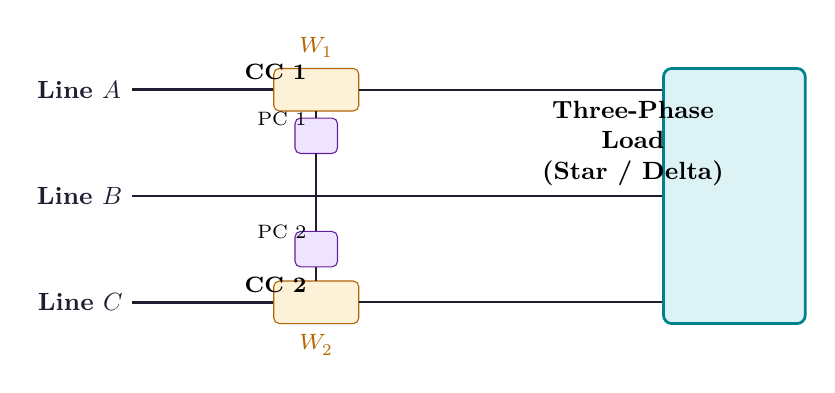
\begin{tikzpicture}[scale=0.9, auto]
  % 3 source lines
  \draw[line, line width=1pt] (0,2.5) node[left, font=\small\bfseries] {Line $A$} -- (2,2.5);
  \draw[line, line width=1pt] (0,1.0) node[left, font=\small\bfseries] {Line $B$} -- (7.5,1.0);
  \draw[line, line width=1pt] (0,-0.5) node[left, font=\small\bfseries] {Line $C$} -- (2,-0.5);

  % Wattmeter 1
  \draw[fill=hdramber, draw=myamber, rounded corners=2pt] (2,2.2) rectangle (3.2,2.8) node[midway, font=\footnotesize\bfseries] {CC 1};
  \draw[line] (3.2,2.5) -- (7.5,2.5);
  \draw[fill=hdrpurple, draw=mypurple, rounded corners=2pt] (2.3,1.6) rectangle (2.9,2.1) node[midway, font=\scriptsize] {PC 1};
  \draw[line] (2.6,2.2) -- (2.6,2.1);
  \draw[line] (2.6,1.6) -- (2.6,1.0);

  % Wattmeter 2
  \draw[fill=hdramber, draw=myamber, rounded corners=2pt] (2,-0.8) rectangle (3.2,-0.2) node[midway, font=\footnotesize\bfseries] {CC 2};
  \draw[line] (3.2,-0.5) -- (7.5,-0.5);
  \draw[fill=hdrpurple, draw=mypurple, rounded corners=2pt] (2.3,0.0) rectangle (2.9,0.5) node[midway, font=\scriptsize] {PC 2};
  \draw[line] (2.6,-0.2) -- (2.6,0.0);
  \draw[line] (2.6,0.5) -- (2.6,1.0);

  % Load block
  \draw[fill=hdrteal, draw=myteal, line width=1pt, rounded corners=3pt] (7.5,-0.8) rectangle (9.5,2.8) node[midway, align=center, font=\small\bfseries] {Three-Phase\\Load\\(Star / Delta)};
  
  \node[font=\footnotesize\bfseries, color=myamber] at (2.6,3.1) {$W_1$};
  \node[font=\footnotesize\bfseries, color=myamber] at (2.6,-1.1) {$W_2$};
\end{tikzpicture}
\end{tcolorbox}

\begin{tcolorbox}[formulabox, title={\textbf{Two-Wattmeter Power and Power Factor Relations}}]
Under balanced sinusoidal conditions with line-to-line voltage $V_L$, line current $I_L$, and load power factor angle $\phi$:
\begin{equation}
  W_1 = V_L I_L \cos(30^\circ - \phi), \qquad W_2 = V_L I_L \cos(30^\circ + \phi)
\end{equation}
\begin{enumerate}[leftmargin=*, itemsep=2pt, topsep=1pt]
  \item \textbf{Total Active Power ($P$):}
  \begin{equation}
    P = W_1 + W_2 = V_L I_L [\cos(30^\circ - \phi) + \cos(30^\circ + \phi)] = \sqrt{3} V_L I_L \cos\phi
  \end{equation}
  \item \textbf{Total Reactive Power ($Q$):}
  \begin{equation}
    W_1 - W_2 = V_L I_L [\cos(30^\circ - \phi) - \cos(30^\circ + \phi)] = V_L I_L \sin\phi \implies Q = \sqrt{3}(W_1 - W_2)
  \end{equation}
  \item \textbf{Power Factor Angle ($\phi$):}
  \begin{equation}
    \tan\phi = \sqrt{3} \frac{W_1 - W_2}{W_1 + W_2} \implies \text{PF} = \cos\phi = \cos\left[ \tan^{-1}\left( \sqrt{3}\frac{W_1 - W_2}{W_1 + W_2} \right) \right]
  \end{equation}
\end{enumerate}
\end{tcolorbox}

\newpage
% ===============================================================================
% MANDATORY QUICK REVISION PAGE
% ===============================================================================
\begin{center}
  {\large\bfseries\color{myred} Quick Revision --- Module 2}\\[3pt]
  {\small\color{mydark} Fourier Analysis and Three-Phase Unbalanced Systems $|$ EC304}
\end{center}
\noindent{\color{myred}\rule{\linewidth}{1.2pt}}
\vspace{4pt}

\begin{tcolorbox}[formulabox, title={\textbf{Key Formulas and Network Relations at a Glance}}]
\renewcommand{\arraystretch}{1.35}
\begin{tabularx}{\linewidth}{B{5.0cm} X}
Trigonometric Fourier Form & $f(t) = a_0 + \sum_{n=1}^\infty [a_n \cos(n\omega_0 t) + b_n \sin(n\omega_0 t)]$ \\[4pt]
Exponential Fourier Form & $f(t) = \sum_{n=-\infty}^\infty C_n e^{j n \omega_0 t}, \quad C_n = \frac{a_n - j b_n}{2}$ \\[4pt]
True RMS Voltage & $V_{\text{rms}} = \sqrt{V_0^2 + \sum_{n=1}^\infty V_{n,\text{rms}}^2}$ \\[4pt]
Average Non-Sinusoidal Power & $P = V_0 I_0 + \sum_{n=1}^\infty V_{n,\text{rms}} I_{n,\text{rms}} \cos(\phi_n)$ \\[4pt]
True Power Factor & $\text{PF} = \frac{P}{S} = \frac{I_{1,\text{rms}}}{I_{\text{rms}}} \cos\phi_1$ \\[4pt]
Total Harmonic Distortion & $\text{THD} = \frac{\sqrt{\sum_{n=2}^\infty I_{n,\text{rms}}^2}}{I_{1,\text{rms}}}$ \\[4pt]
Complex Operator $a$ & $a = e^{j 120^\circ} = -\frac{1}{2} + j\frac{\sqrt{3}}{2}, \quad 1 + a + a^2 = 0$ \\[4pt]
Zero-Sequence Current & $\mathbf{I}_{a0} = \frac{\mathbf{I}_a + \mathbf{I}_b + \mathbf{I}_c}{3} = \frac{\mathbf{I}_n}{3}$ \\[4pt]
Two-Wattmeter Total Power & $P_{\text{total}} = W_1 + W_2 = \sqrt{3} V_L I_L \cos\phi$ \\[4pt]
Two-Wattmeter Power Factor & $\tan\phi = \sqrt{3} \frac{W_1 - W_2}{W_1 + W_2}$ \\[4pt]
\end{tabularx}
\end{tcolorbox}

\begin{tcolorbox}[defbox, title={\textbf{One-Line Definitions}}]
\begin{itemize}[leftmargin=*, itemsep=2pt, topsep=0pt]
  \item \textbf{Harmonic Frequency:} An integer multiple ($n\omega_0$) of the fundamental repetition frequency of a periodic wave.
  \item \textbf{Half-Wave Symmetry:} Condition $f(t \pm T/2) = -f(t)$, ensuring complete cancellation of all even harmonic orders.
  \item \textbf{Line Spectrum:} A discrete graphical plot of harmonic component amplitudes and phase shifts versus frequency.
  \item \textbf{Harmonic Impedance:} The frequency-dependent impedance of a circuit evaluated specifically at harmonic frequency $n\omega_0$.
  \item \textbf{Distortion Power ($D$):} The component of apparent power caused strictly by harmonic cross-frequencies, measured in VA.
  \item \textbf{Displacement Factor:} The cosine of the fundamental phase angle ($\cos\phi_1$), measuring fundamental displacement.
  \item \textbf{Symmetrical Components:} Three balanced phasor sets (positive, negative, zero) replacing an unbalanced three-phase system.
  \item \textbf{Neutral Shift Voltage:} The potential difference appearing between floating load neutral and source star neutral in unbalanced loads.
  \item \textbf{Two-Wattmeter Method:} A standard method using two power meters to measure total power in any three-phase three-wire system.
  \item \textbf{Parseval's Theorem:} Mathematical relation stating total energy is conserved between time and continuous frequency domains.
\end{itemize}
\end{tcolorbox}

\begin{tcolorbox}[exambox, title={\textbf{Frequently Asked / Viva Questions}}]
\begin{enumerate}[topsep=0pt, label=\textbf{Q\arabic*.}, itemsep=5pt]
  \item \Q{What harmonics are present in a periodic waveform possessing Half-Wave Symmetry?}
  A waveform with half-wave symmetry ($f(t \pm T/2) = -f(t)$) contains strictly odd harmonics ($n = 1, 3, 5, \dots$). The DC component ($a_0$) and all even harmonics ($a_{2k}, b_{2k}$) are identically zero.

  \item \Q{Why does a non-sinusoidal voltage produce an active power contribution only with currents of the identical harmonic order?}
  Because the time-average product of two sinusoids of differing frequencies over the fundamental period is identically zero: $\int_0^T \cos(m\omega_0 t)\cos(n\omega_0 t)dt = 0$ for $m \ne n$. Active power is generated exclusively by voltage and current terms belonging to the same harmonic frequency.

  \item \Q{Can zero-sequence currents flow in a balanced or unbalanced 3-phase 3-wire system? Explain.}
  No. In any 3-phase 3-wire system, by KCL, the sum of line currents must be zero ($\mathbf{I}_a + \mathbf{I}_b + \mathbf{I}_c = 0$). Since zero-sequence current is $\mathbf{I}_{a0} = \frac{1}{3}(\mathbf{I}_a + \mathbf{I}_b + \mathbf{I}_c)$, it is strictly zero. A neutral or ground path is required for zero-sequence current to exist.

  \item \Q{What does it mean if one wattmeter reads negative in the two-wattmeter method?}
  A negative reading occurs when the load power factor is less than $0.5$ ($\phi > 60^\circ$). In that case, $W_2 = V_L I_L \cos(30^\circ + \phi)$ becomes negative. Total power is still the algebraic sum $W_1 + W_2$.

  \item \Q{What are the readings of the two wattmeters at unity power factor ($\cos\phi = 1$)?}
  At unity power factor, $\phi = 0^\circ$. Thus, $W_1 = V_L I_L \cos(30^\circ) = \frac{\sqrt{3}}{2}V_L I_L$ and $W_2 = V_L I_L \cos(30^\circ) = \frac{\sqrt{3}}{2}V_L I_L$. Both wattmeters read identical positive values ($W_1 = W_2 = P/2$).

  \item \Q{What are the readings of the two wattmeters at zero power factor ($\cos\phi = 0$)?}
  At zero power factor, $\phi = 90^\circ$. Then $W_1 = V_L I_L \cos(-60^\circ) = 0.5 V_L I_L$ and $W_2 = V_L I_L \cos(120^\circ) = -0.5 V_L I_L$. The wattmeters have equal magnitudes but opposite signs ($W_1 = -W_2$), yielding net active power $P = W_1 + W_2 = 0$.

  \item \Q{State the relationship between Total Harmonic Distortion (THD) and Distortion Factor.}
  The distortion factor $\mu = I_{1,\text{rms}} / I_{\text{rms}}$ relates to THD by $\mu = \frac{1}{\sqrt{1 + \text{THD}^2}}$. As harmonic distortion increases, the distortion factor decreases below unity, degrading true power factor.

  \item \Q{What is the physical meaning of the complex operator $a = e^{j 120^\circ}$?}
  The operator $a$ represents a counter-clockwise phase rotation of $120^\circ$ ($2\pi/3\text{ radians}$) without altering the magnitude of the phasor. Multiplying by $a^2$ rotates by $240^\circ$.

  \item \Q{How does Millman's Theorem find the neutral shift in an unbalanced 3-phase star circuit?}
  Millman's theorem treats the 3 phase voltages as parallel branches connected to neutral. The star point voltage is $\mathbf{V}_{N'N} = (\sum \mathbf{V}_k \mathbf{Y}_k) / \sum \mathbf{Y}_k$, directly yielding the shift in neutral potential.

  \item \Q{Distinguish between continuous and discrete Fourier spectra.}
  A discrete spectrum consists of isolated impulses at integer multiples of fundamental frequency $n\omega_0$, characteristic of periodic signals. A continuous spectrum is a continuous function of $\omega$ spanning all frequencies, characteristic of non-periodic transient energy pulses.
\end{enumerate}
\end{tcolorbox}

\begin{tcolorbox}[tikzbox, title={\textbf{Summary Matrix: Waveform Symmetries and Two-Wattmeter Diagnostic Rules}}]
\par\vspace{4pt}\noindent
\begingroup
\setlength{\tabcolsep}{4.5pt}
\setlength{\extrarowheight}{3pt}
\renewcommand{\arraystretch}{1.35}
\begin{tabularx}{\linewidth}{|B{3.2cm}|B{3.8cm}|Y|}
\hline
\multicolumn{1}{|c|}{\textbf{Operating Condition}} & \multicolumn{1}{c|}{\textbf{Wattmeter Relationship}} & \multicolumn{1}{c|}{\textbf{Power Factor / Significance}} \\
\hline
$\phi = 0^\circ$ (Resistive) & $W_1 = W_2 > 0$ & $\text{PF} = 1.0$; identical positive readings. \\
\hline
$\phi = 60^\circ$ & $W_1 > 0, \quad W_2 = 0$ & $\text{PF} = 0.5$; meter 2 reads exactly zero. \\
\hline
$\phi > 60^\circ$ (Lagging) & $W_1 > 0, \quad W_2 < 0$ & $\text{PF} < 0.5$; meter 2 reverses deflection. \\
\hline
$\phi = 90^\circ$ (Pure Reactive) & $W_1 = -W_2$ & $\text{PF} = 0$; net active power is strictly zero. \\
\hline
Unbalanced 3-Wire System & $W_1 + W_2 = P_{\text{total}}$ & Valid regardless of load unbalance or power factor. \\
\hline
\end{tabularx}
\endgroup
\end{tcolorbox}


% -- Module 3 -----------------------------------------------------------------
\modulestart{3}{Singularity Functions and Waveform Synthesis}

\section{Singularity Functions and Waveform Synthesis}

Singularity functions (also referred to as switching functions or test signals) are a family of mathematical idealizations exhibiting discontinuities or discontinuous derivatives. In linear circuit theory, they model switching actions, sharp current/voltage pulses, and sudden transients.

\subsection{Standard Singularity Functions}

\begin{tcolorbox}[defbox, title={\textbf{Definitions of Core Singularity Functions}}]
\begin{enumerate}[leftmargin=*, itemsep=4pt]
  \item \textbf{Unit Step Function $u(t)$:} Models the instantaneous closing or opening of an ideal switch at $t = 0$:
  \begin{equation}
    u(t) = \begin{cases} 0, & t < 0 \\ 1, & t > 0 \end{cases} \qquad \text{Delayed: } u(t - t_0) = \begin{cases} 0, & t < t_0 \\ 1, & t > t_0 \end{cases}
  \end{equation}
  \item \textbf{Unit Impulse (Dirac Delta) Function $\delta(t)$:} Defined as the distributional derivative of the unit step function:
  \begin{equation}
    \delta(t) = \frac{du(t)}{dt}, \quad \delta(t) = 0 \text{ for } t \ne 0, \quad \int_{-\infty}^{\infty} \delta(t)\,dt = 1
  \end{equation}
  \textbf{Sifting (Sampling) Property:}
  \begin{equation}
    \int_{-\infty}^{\infty} f(t)\,\delta(t - t_0)\,dt = f(t_0)
  \end{equation}
  \item \textbf{Unit Ramp Function $r(t)$:} Represents a linearly growing excitation starting at $t=0$:
  \begin{equation}
    r(t) = \int_{-\infty}^t u(\tau)\,d\tau = t\,u(t) = \begin{cases} 0, & t < 0 \\ t, & t \ge 0 \end{cases}
  \end{equation}
  \item \textbf{Unit Doublet $\delta'(t)$:} The time derivative of the unit impulse function:
  \begin{equation}
    \delta'(t) = \frac{d\delta(t)}{dt}, \qquad \int_{-\infty}^\infty f(t)\,\delta'(t - t_0)\,dt = -f'(t_0)
  \end{equation}
\end{enumerate}
\end{tcolorbox}

\begin{tcolorbox}[formulabox, title={\textbf{Hierarchy of Singularity Functions}}]
The standard singularity functions form a continuous calculus chain linked by differentiation and integration:
\begin{equation}
  \cdots \xleftarrow{\frac{d}{dt}} \delta'(t) \xleftarrow{\frac{d}{dt}} \delta(t) \xleftarrow{\frac{d}{dt}} u(t) \xleftarrow{\frac{d}{dt}} r(t) \xleftarrow{\frac{d}{dt}} \frac{t^2}{2}u(t) \cdots
\end{equation}
\end{tcolorbox}

\subsection{Waveform Synthesis Technique}

Any arbitrary piecewise-linear or stepped signal can be synthesized systematically as a linear algebraic sum of delayed ramp functions and delayed step functions:
\begin{equation}
  v(t) = \sum_{k=0}^{N} \Delta m_k\, r(t - t_k) + \sum_{j=0}^{M} \Delta v_j\, u(t - t_j)
\end{equation}
where $\Delta m_k = m_k - m_{k-1}$ is the change in slope at breakpoint $t_k$, and $\Delta v_j$ is the abrupt jump in amplitude at breakpoint $t_j$.

\begin{tcolorbox}[tikzbox, title={\textbf{TikZ Schematic: Synthesis of a Trapezoidal Pulse from Singularity Functions}}]
\begin{center}
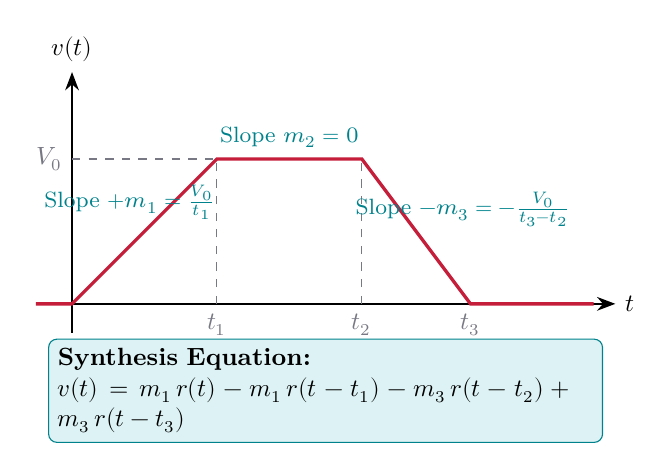
\begin{tikzpicture}[scale=0.92, every node/.style={font=\small}]
  % Axes
  \draw[-Stealth, thick] (-0.5,0) -- (7.5,0) node[right] {$t$};
  \draw[-Stealth, thick] (0,-0.4) -- (0,3.2) node[above] {$v(t)$};

  % Trapezoid waveform
  \draw[very thick, color=myred] (-0.5,0) -- (0,0) -- (2,2) -- (4,2) -- (5.5,0) -- (7.2,0);

  % Dashed projection lines
  \draw[dashed, color=mydark!60] (2,0) node[below] {$t_1$} -- (2,2);
  \draw[dashed, color=mydark!60] (4,0) node[below] {$t_2$} -- (4,2);
  \draw[dashed, color=mydark!60] (5.5,0) node[below] {$t_3$} -- (5.5,0);
  \draw[dashed, color=mydark!60] (0,2) node[left] {$V_0$} -- (2,2);

  % Annotations
  \node[color=myteal, font=\footnotesize] at (0.8, 1.4) {Slope $+m_1 = \frac{V_0}{t_1}$};
  \node[color=myteal, font=\footnotesize] at (3.0, 2.3) {Slope $m_2 = 0$};
  \node[color=myteal, font=\footnotesize] at (5.4, 1.3) {Slope $-m_3 = -\frac{V_0}{t_3 - t_2}$};

  % Equation Box
  \node[draw=myteal, fill=hdrteal, rounded corners=3pt, text width=6.8cm, align=left] at (3.5, -1.2) {
    \textbf{Synthesis Equation:}\\
    $v(t) = m_1\,r(t) - m_1\,r(t-t_1) - m_3\,r(t-t_2) + m_3\,r(t-t_3)$
  };
\end{tikzpicture}
\end{center}
\end{tcolorbox}

\begin{tcolorbox}[examplebox, title={\textbf{Step-by-Step Example: Waveform Synthesis and its Transform}}]
\textbf{Problem:} Express a triangular pulse that rises linearly from $0$ to $10\text{ V}$ between $t=0$ and $t=2\text{ s}$, and drops instantaneously to zero at $t=2\text{ s}$. Determine its Laplace transform.

\textbf{Solution:}
\begin{enumerate}[leftmargin=*]
  \item Between $t=0$ and $t=2$, the waveform has a constant slope $m_1 = \frac{10 - 0}{2 - 0} = +5\text{ V/s}$. It starts at $t=0$, represented as $5\,r(t)$.
  \item At $t=2\text{ s}$, the ramp must be cancelled by subtracting an identical ramp of slope $5$: $-5\,r(t-2)$.
  \item At $t=2\text{ s}$, the voltage must also jump downwards instantaneously by $-10\text{ V}$ to reach $0$: $-10\,u(t-2)$.
  \item Synthesized time-domain expression:
  \begin{equation}
    v(t) = 5\,r(t) - 5\,r(t-2) - 10\,u(t-2)
  \end{equation}
  \item Applying the time-shifting property of the Laplace transform:
  \begin{equation}
    V(s) = \frac{5}{s^2} - \frac{5}{s^2}\,e^{-2s} - \frac{10}{s}\,e^{-2s} = \frac{5}{s^2}\left[1 - e^{-2s}(1 + 2s)\right]
  \end{equation}
\end{enumerate}
\end{tcolorbox}

% ===============================================================================
% SECTION 2: THE LAPLACE TRANSFORM AND PROPERTIES
% ===============================================================================
\section{The Laplace Transform and Operational Theorems}

The unilateral (one-sided) Laplace transform is an essential mathematical tool for solving linear, time-invariant (LTI) differential equations with non-zero initial boundary conditions.

\subsection{Definition and Region of Convergence}

\begin{tcolorbox}[defbox, title={\textbf{Unilateral Laplace Transform}}]
Let $f(t)$ be a continuous or piecewise-continuous function defined for $t \ge 0$. The unilateral Laplace transform $\mathcal{L}\{f(t)\} = F(s)$ is:
\begin{equation}
  F(s) = \int_{0^-}^\infty f(t)\,e^{-st}\,dt
\end{equation}
where $s = \sigma + j\omega$ is the complex frequency variable. The lower integration limit $0^- \equiv \lim_{\epsilon \to 0^+} (0 - \epsilon)$ ensures that singularity functions (such as $\delta(t)$) acting at $t=0$ are rigorously integrated and accounted for.
\end{tcolorbox}

\subsection{Operational Theorems for Circuit Analysis}

\par\vspace{6pt}\noindent
\begingroup
\setlength{\tabcolsep}{5pt}
\setlength{\extrarowheight}{3pt}
\renewcommand{\arraystretch}{1.38}
\begin{tabularx}{\linewidth}{|B{3.4cm}|B{3.2cm}|Y|}
\hline
\multicolumn{1}{|c|}{\textbf{Property / Theorem}} & \multicolumn{1}{c|}{\textbf{Time Domain $f(t)$}} & \multicolumn{1}{c|}{\textbf{Frequency Domain $F(s)$}} \\
\hline
Linearity & $a_1 f_1(t) + a_2 f_2(t)$ & $a_1 F_1(s) + a_2 F_2(s)$ \\
\hline
First Shifting (Frequency) & $e^{-at} f(t)$ & $F(s + a)$ \\
\hline
Second Shifting (Time) & $f(t - t_0)\,u(t - t_0)$ & $e^{-s t_0} F(s) \quad (t_0 \ge 0)$ \\
\hline
Time Differentiation (1st) & $\dfrac{df(t)}{dt}$ & $s F(s) - f(0^-)$ \\
\hline
Time Differentiation (2nd) & $\dfrac{d^2f(t)}{dt^2}$ & $s^2 F(s) - s f(0^-) - f'(0^-)$ \\
\hline
Time Integration & $\displaystyle\int_{0^-}^t f(\tau)\,d\tau$ & $\dfrac{F(s)}{s}$ \\
\hline
Frequency Differentiation & $t\,f(t)$ & $-\dfrac{d}{ds}F(s)$ \\
\hline
Time Convolution & $f_1(t) * f_2(t)$ & $F_1(s) \cdot F_2(s)$ \\
\hline
Initial Value Theorem & $\displaystyle\lim_{t \to 0^+} f(t)$ & $\displaystyle\lim_{s \to \infty} s F(s)$ \quad (if limit exists) \\
\hline
Final Value Theorem & $\displaystyle\lim_{t \to \infty} f(t)$ & $\displaystyle\lim_{s \to 0} s F(s)$ \quad (poles of $sF(s)$ in LHP) \\
\hline
Periodic Function ($T$) & $f(t) = f(t + T)$ & $\dfrac{1}{1 - e^{-sT}} \displaystyle\int_0^T f(t) e^{-st}\,dt$ \\
\hline
\end{tabularx}
\endgroup
\vspace{12pt}

\begin{tcolorbox}[masonbox, title={\textbf{Critical Examination Note: Validity of the Final Value Theorem (FVT)}}]
The Final Value Theorem $\lim_{t \to \infty} f(t) = \lim_{s \to 0} s F(s)$ is valid \textbf{if and only if} the function $f(t)$ possesses a finite, stable steady-state limit as $t \to \infty$. Mathematically, this requires that all poles of $s F(s)$ reside strictly in the open left-half of the $s$-plane ($\text{Re}(s) < 0$).
\begin{itemize}[leftmargin=*]
  \item For $f(t) = \sin(\omega_0 t)$, $F(s) = \frac{\omega_0}{s^2 + \omega_0^2}$. Here $sF(s) = \frac{s\omega_0}{s^2 + \omega_0^2}$. Evaluating $\lim_{s \to 0} sF(s) = 0$, but $\lim_{t \to \infty}\sin(\omega_0 t)$ does not exist (it oscillates indefinitely). FVT fails because poles are on the $j\omega$-axis!
\end{itemize}
\end{tcolorbox}

\subsection{Standard Laplace Transform Pairs}

\par\vspace{6pt}\noindent
\begingroup
\setlength{\tabcolsep}{5pt}
\setlength{\extrarowheight}{2.5pt}
\renewcommand{\arraystretch}{1.35}
\begin{tabularx}{\linewidth}{|B{3.2cm}|B{3.0cm}|B{3.2cm}|Y|}
\hline
\multicolumn{1}{|c|}{\textbf{Signal $f(t)$}} & \multicolumn{1}{c|}{\textbf{$F(s)$}} & \multicolumn{1}{c|}{\textbf{Signal $f(t)$}} & \multicolumn{1}{c|}{\textbf{$F(s)$}} \\
\hline
$\delta(t)$ & $1$ & $u(t)$ & $\dfrac{1}{s}$ \\
\hline
$t\,u(t)$ & $\dfrac{1}{s^2}$ & $t^n\,u(t)$ & $\dfrac{n!}{s^{n+1}}$ \\
\hline
$e^{-at}\,u(t)$ & $\dfrac{1}{s + a}$ & $t\,e^{-at}\,u(t)$ & $\dfrac{1}{(s + a)^2}$ \\
\hline
$\sin(\omega t)\,u(t)$ & $\dfrac{\omega}{s^2 + \omega^2}$ & $\cos(\omega t)\,u(t)$ & $\dfrac{s}{s^2 + \omega^2}$ \\
\hline
$e^{-at}\sin(\omega t)\,u(t)$ & $\dfrac{\omega}{(s + a)^2 + \omega^2}$ & $e^{-at}\cos(\omega t)\,u(t)$ & $\dfrac{s + a}{(s + a)^2 + \omega^2}$ \\
\hline
\end{tabularx}
\endgroup
\vspace{12pt}

% ===============================================================================
% SECTION 3: INVERSE LAPLACE TRANSFORM AND PARTIAL FRACTIONS
% ===============================================================================
\section{Inverse Laplace Transform and Partial Fraction Expansion}

In network transient problems, the $s$-domain response is generally obtained as a rational transfer function $F(s) = \frac{P(s)}{Q(s)}$, where $P(s)$ and $Q(s)$ are polynomials in $s$ with real coefficients, and $\text{deg}(P) < \text{deg}(Q)$ (strictly proper).

\subsection{Decomposition Methodologies}

\begin{tcolorbox}[defbox, title={\textbf{Three Cases of Partial Fraction Expansion}}]
\begin{enumerate}[leftmargin=*, itemsep=4pt]
  \item \textbf{Case I: Distinct Real Roots (Simple Poles)}
  \begin{equation}
    F(s) = \frac{P(s)}{(s - p_1)(s - p_2)\cdots(s - p_n)} = \sum_{k=1}^n \frac{A_k}{s - p_k}
  \end{equation}
  The residues $A_k$ are evaluated by Heaviside's cover-up rule:
  \begin{equation}
    A_k = \lim_{s \to p_k} (s - p_k)\,F(s) \implies f(t) = \sum_{k=1}^n A_k\,e^{p_k t}\,u(t)
  \end{equation}

  \item \textbf{Case II: Repeated Real Roots (Multiple Poles of Order $m$)}
  \begin{equation}
    F(s) = \frac{P(s)}{(s - p)^m\,Q_1(s)} = \frac{B_m}{(s - p)^m} + \frac{B_{m-1}}{(s - p)^{m-1}} + \cdots + \frac{B_1}{s - p} + \cdots
  \end{equation}
  where the coefficients are given by:
  \begin{equation}
    B_{m-k} = \frac{1}{k!}\lim_{s \to p} \frac{d^k}{ds^k} \left[(s - p)^m\,F(s)\right], \quad k = 0, 1, \dots, m-1
  \end{equation}

  \item \textbf{Case III: Complex Conjugate Poles ($s = -\alpha \pm j\beta$)}
  \begin{equation}
    F(s) = \frac{C s + D}{(s + \alpha)^2 + \beta^2} = \frac{C(s + \alpha) + (D - C\alpha)}{(s + \alpha)^2 + \beta^2}
  \end{equation}
  The inverse transform yields a damped sinusoid:
  \begin{equation}
    f(t) = C e^{-\alpha t}\cos(\beta t) + \frac{D - C\alpha}{\beta} e^{-\alpha t}\sin(\beta t) = M e^{-\alpha t}\cos(\beta t - \theta)
  \end{equation}
  where $M = \sqrt{C^2 + \left(\frac{D - C\alpha}{\beta}\right)^2}$ and $\theta = \tan^{-1}\left(\frac{D - C\alpha}{\beta C}\right)$.
\end{enumerate}
\end{tcolorbox}

% ===============================================================================
% SECTION 4: EVALUATION OF INITIAL CONDITIONS
% ===============================================================================
\section{Evaluation of Initial Conditions in Electrical Networks}

Evaluating initial conditions at the switching instant ($t = 0^-$ and $t = 0^+$) is an absolute prerequisite for setting up transient differential equations and their Laplace counterparts.

\subsection{Physical Boundary and Continuity Principles}

\begin{tcolorbox}[defbox, title={\textbf{Energy Continuity Postulates}}]
\begin{enumerate}[leftmargin=*]
  \item \textbf{Conservation of Inductor Flux Linkage:} An inductor stores magnetic energy $W_m = \frac{1}{2} L i_L^2$. An instantaneous discontinuity in $i_L(t)$ requires infinite voltage ($v_L = L \frac{di}{dt} \to \infty$) and infinite instantaneous power, which is physically impossible in passive circuits without impulse voltage sources. Therefore:
  \begin{equation}
    i_L(0^+) = i_L(0^-)
  \end{equation}
  \item \textbf{Conservation of Capacitor Electric Charge:} A capacitor stores electrostatic energy $W_e = \frac{1}{2} C v_C^2$. An instantaneous discontinuity in $v_C(t)$ requires infinite current ($i_C = C \frac{dv_C}{dt} \to \infty$), which is physically impossible in passive circuits without impulse current sources. Therefore:
  \begin{equation}
    v_C(0^+) = v_C(0^-)
  \end{equation}
\end{enumerate}
\end{tcolorbox}

\subsection{Equivalent Circuits at $t=0^-$ and $t=0^+$}

\par\vspace{6pt}\noindent
\begingroup
\setlength{\tabcolsep}{4.5pt}
\setlength{\extrarowheight}{2.5pt}
\renewcommand{\arraystretch}{1.30}
\begin{tabularx}{\linewidth}{|B{2.2cm}|B{3.4cm}|B{3.8cm}|Y|}
\hline
\textbf{Element} & \textbf{DC Steady State ($t = 0^-$)} & \textbf{At $t = 0^+$ (With Initial State)} & \textbf{At $t = 0^+$ (Zero Initial State)} \\
\hline
Resistor ($R$) & Resistor $R$ ($v_R = i_R R$) & Resistor $R$ ($v_R = i_R R$) & Resistor $R$ ($v_R = i_R R$) \\
\hline
Inductor ($L$) & Short Circuit ($v_L = 0$) & Current Source $I_0 = i_L(0^-)$ & Open Circuit ($i_L(0^+) = 0$) \\
\hline
Capacitor ($C$) & Open Circuit ($i_C = 0$) & Voltage Source $V_0 = v_C(0^-)$ & Short Circuit ($v_C(0^+) = 0$) \\
\hline
\end{tabularx}
\endgroup
\vspace{12pt}

\subsection{Evaluation of Higher Derivatives at $t = 0^+$}

To evaluate higher-order derivatives such as $\frac{di}{dt}(0^+)$, $\frac{dv_C}{dt}(0^+)$, and $\frac{d^2i}{dt^2}(0^+)$:
\begin{enumerate}[leftmargin=*]
  \item Write the loop KVL and nodal KCL equations for $t > 0$ containing derivative terms:
  \begin{equation}
    v_L(t) = L\,\frac{di_L(t)}{dt} \implies \left.\frac{di_L}{dt}\right|_{t=0^+} = \frac{v_L(0^+)}{L}
  \end{equation}
  \begin{equation}
    i_C(t) = C\,\frac{dv_C(t)}{dt} \implies \left.\frac{dv_C}{dt}\right|_{t=0^+} = \frac{i_C(0^+)}{C}
  \end{equation}
  \item Calculate $v_L(0^+)$ and $i_C(0^+)$ directly by evaluating the network loop/node equations at the instant $t = 0^+$ using the known boundary values $i_L(0^+)$ and $v_C(0^+)$.
  \item Differentiate the general differential equation with respect to $t$, and evaluate the resulting relation at $t = 0^+$ to find the second derivative $\frac{d^2i}{dt^2}(0^+)$.
\end{enumerate}

\begin{tcolorbox}[examplebox, title={\textbf{Worked Example: Complete Evaluation of Initial Boundary Derivatives}}]
\textbf{Problem:} In a series RLC circuit ($R=10\,\Omega, L=1\text{ H}, C=0.1\text{ F}$), a DC voltage $V = 100\text{ V}$ is suddenly applied at $t=0$ by closing a switch. The circuit had no initial energy ($i_L(0^-)=0, v_C(0^-)=0$). Find $i(0^+)$, $\frac{di}{dt}(0^+)$, and $\frac{d^2i}{dt^2}(0^+)$.

\textbf{Solution:}
\begin{enumerate}[leftmargin=*]
  \item \textbf{At $t = 0^+$:}
  Due to continuity of inductor current, $i(0^+) = i_L(0^-) = 0\text{ A}$.
  Due to continuity of capacitor voltage, $v_C(0^+) = v_C(0^-) = 0\text{ V}$.
  \item \textbf{First derivative $\frac{di}{dt}(0^+)$:}
  Applying KVL around the loop for $t \ge 0$:
  \begin{equation}
    R\,i(t) + L\,\frac{di(t)}{dt} + v_C(t) = V
  \end{equation}
  Evaluating this at $t = 0^+$:
  \begin{equation}
    R\,i(0^+) + L\left.\frac{di}{dt}\right|_{t=0^+} + v_C(0^+) = V \implies 10(0) + 1 \cdot \left.\frac{di}{dt}\right|_{t=0^+} + 0 = 100
  \end{equation}
  \begin{equation}
    \left.\frac{di}{dt}\right|_{t=0^+} = \frac{100 - 0 - 0}{1} = 100\text{ A/s}
  \end{equation}
  \item \textbf{Second derivative $\frac{d^2i}{dt^2}(0^+)$:}
  Differentiating the KVL equation with respect to time $t$:
  \begin{equation}
    R\,\frac{di(t)}{dt} + L\,\frac{d^2i(t)}{dt^2} + \frac{dv_C(t)}{dt} = 0 \implies R\,\frac{di}{dt} + L\,\frac{d^2i}{dt^2} + \frac{i(t)}{C} = 0
  \end{equation}
  Evaluating at $t = 0^+$:
  \begin{equation}
    10(100) + 1 \cdot \left.\frac{d^2i}{dt^2}\right|_{t=0^+} + \frac{0}{0.1} = 0 \implies \left.\frac{d^2i}{dt^2}\right|_{t=0^+} = -1000\text{ A/s}^2
  \end{equation}
\end{enumerate}
\end{tcolorbox}

% ===============================================================================
% SECTION 5: TRANSFORMED S-DOMAIN CIRCUIT MODELS
% ===============================================================================
\section{Transformed $s$-Domain Circuit Models}

Instead of formulating differential equations in the time domain and then taking the transform, we can directly map each physical circuit element into its transformed algebraic $s$-domain model containing initial conditions.

\subsection{Derivation of Element Equivalent Circuits}

\begin{tcolorbox}[defbox, title={\textbf{Mathematical Derivation of $s$-Domain Models}}]
\begin{enumerate}[leftmargin=*]
  \item \textbf{Resistor ($R$):}
  \begin{equation}
    v(t) = R\,i(t) \iff V(s) = R\,I(s) \qquad \text{Impedance: } Z_R(s) = R
  \end{equation}
  \item \textbf{Inductor ($L$):}
  \begin{equation}
    v_L(t) = L\,\frac{di_L}{dt} \iff V_L(s) = sL\,I_L(s) - L\,i_L(0^-)
  \end{equation}
  \begin{itemize}
    \item \textbf{Thevenin Form (Series):} An impedance $sL$ in series with an opposing voltage source of magnitude $L\,i_L(0^-)$ (positive terminal at the current entry).
    \item \textbf{Norton Form (Parallel):} Solving for $I_L(s)$:
    \begin{equation}
      I_L(s) = \frac{V_L(s)}{sL} + \frac{i_L(0^-)}{s}
    \end{equation}
    An admittance $\frac{1}{sL}$ in parallel with an independent current source $\frac{i_L(0^-)}{s}$ pointing in the direction of $i_L(t)$.
  \end{itemize}
  \item \textbf{Capacitor ($C$):}
  \begin{equation}
    i_C(t) = C\,\frac{dv_C}{dt} \iff I_C(s) = sC\,V_C(s) - C\,v_C(0^-)
  \end{equation}
  \begin{itemize}
    \item \textbf{Norton Form (Parallel):} An admittance $sC$ in parallel with an independent current source $C\,v_C(0^-)$ directed towards the positive terminal.
    \item \textbf{Thevenin Form (Series):} Solving for $V_C(s)$:
    \begin{equation}
      V_C(s) = \frac{I_C(s)}{sC} + \frac{v_C(0^-)}{s}
    \end{equation}
    An impedance $\frac{1}{sC}$ in series with a voltage source $\frac{v_C(0^-)}{s}$ maintaining the polarity of $v_C(0^-)$.
  \end{itemize}
\end{enumerate}
\end{tcolorbox}

\begin{tcolorbox}[tikzbox, title={\textbf{TikZ Schematic: Transformed $s$-Domain Circuit Equivalents with Initial Energy}}]
\begin{center}
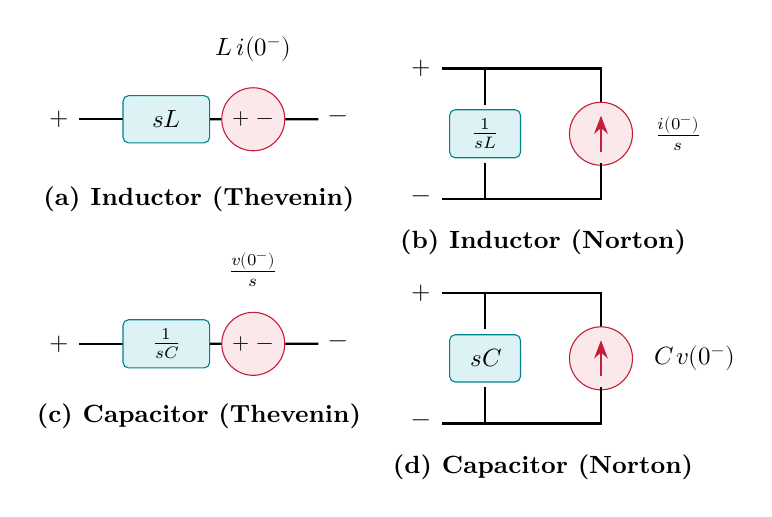
\begin{tikzpicture}[scale=0.92, every node/.style={font=\small}]
  % Inductor Thevenin (Series)
  \draw[thick] (0,2.5) node[left] {$+$} -- (0.6,2.5);
  \node[draw=myteal, fill=hdrteal, minimum width=1.1cm, minimum height=0.6cm, rounded corners=2pt] (ZL) at (1.2,2.5) {$sL$};
  \draw[thick] (ZL.east) -- (2.0,2.5);
  \node[sourcenode, minimum size=0.8cm] (VL) at (2.4,2.5) {};
  \node at (2.4, 2.5) {\footnotesize $+ \,\, -$};
  \node[above=0.2cm of VL] {$L\,i(0^-)$};
  \draw[thick] (VL.east) -- (3.3,2.5) node[right] {$-$};
  \node at (1.65, 1.4) {\textbf{(a) Inductor (Thevenin)}};

  % Inductor Norton (Parallel)
  \draw[thick] (5.0,3.2) node[left] {$+$} -- (5.6,3.2) -- (5.6,2.7);
  \node[draw=myteal, fill=hdrteal, minimum width=0.9cm, minimum height=0.6cm, rounded corners=2pt] (YL) at (5.6,2.3) {$\frac{1}{sL}$};
  \draw[thick] (5.6,1.9) -- (5.6,1.4) -- (5.0,1.4) node[left] {$-$};
  \draw[thick] (5.6,3.2) -- (7.2,3.2) -- (7.2,2.7);
  \node[sourcenode, minimum size=0.8cm] (IL) at (7.2,2.3) {};
  \draw[-Stealth, thick, color=myred] (7.2, 2.05) -- (7.2, 2.55);
  \node[right=0.15cm of IL] {$\frac{i(0^-)}{s}$};
  \draw[thick] (7.2,1.9) -- (7.2,1.4) -- (5.6,1.4);
  \node at (6.4, 0.8) {\textbf{(b) Inductor (Norton)}};

  % Capacitor Thevenin (Series)
  \draw[thick] (0,-0.6) node[left] {$+$} -- (0.6,-0.6);
  \node[draw=myteal, fill=hdrteal, minimum width=1.1cm, minimum height=0.6cm, rounded corners=2pt] (ZC) at (1.2,-0.6) {$\frac{1}{sC}$};
  \draw[thick] (ZC.east) -- (2.0,-0.6);
  \node[sourcenode, minimum size=0.8cm] (VC) at (2.4,-0.6) {};
  \node at (2.4, -0.6) {\footnotesize $+ \,\, -$};
  \node[above=0.2cm of VC] {$\frac{v(0^-)}{s}$};
  \draw[thick] (VC.east) -- (3.3,-0.6) node[right] {$-$};
  \node at (1.65, -1.6) {\textbf{(c) Capacitor (Thevenin)}};

  % Capacitor Norton (Parallel)
  \draw[thick] (5.0,0.1) node[left] {$+$} -- (5.6,0.1) -- (5.6,-0.4);
  \node[draw=myteal, fill=hdrteal, minimum width=0.9cm, minimum height=0.6cm, rounded corners=2pt] (YC) at (5.6,-0.8) {$sC$};
  \draw[thick] (5.6,-1.2) -- (5.6,-1.7) -- (5.0,-1.7) node[left] {$-$};
  \draw[thick] (5.6,0.1) -- (7.2,0.1) -- (7.2,-0.4);
  \node[sourcenode, minimum size=0.8cm] (IC) at (7.2,-0.8) {};
  \draw[-Stealth, thick, color=myred] (7.2, -1.05) -- (7.2, -0.55);
  \node[right=0.15cm of IC] {$C\,v(0^-)$};
  \draw[thick] (7.2,-1.2) -- (7.2,-1.7) -- (5.6,-1.7);
  \node at (6.4, -2.3) {\textbf{(d) Capacitor (Norton)}};
\end{tikzpicture}
\end{center}
\end{tcolorbox}

% ===============================================================================
% SECTION 6: FIRST-ORDER NETWORK TRANSIENTS
% ===============================================================================
\section{Transient Analysis of First-Order Networks (RL and RC)}

First-order circuits contain a single equivalent energy-storage element ($L$ or $C$) and are mathematically governed by linear first-order ordinary differential equations.

\subsection{Series RL Network with DC Step Voltage}

Consider a series connection of resistance $R$ and inductance $L$ excited at $t=0$ by a step voltage $V\,u(t)$ with an initial current $i(0^-) = I_0$.

\begin{tcolorbox}[formulabox, title={\textbf{Mathematical Derivation of RL Response}}]
Applying KVL in the transformed $s$-domain:
\begin{equation}
  \frac{V}{s} = R\,I(s) + sL\,I(s) - L\,I_0 \implies I(s)(R + sL) = \frac{V}{s} + L\,I_0
\end{equation}
Solving for the current transform $I(s)$:
\begin{equation}
  I(s) = \frac{V}{s(sL + R)} + \frac{L\,I_0}{sL + R} = \frac{V/L}{s\left(s + \frac{R}{L}\right)} + \frac{I_0}{s + \frac{R}{L}}
\end{equation}
Decomposing the first term via partial fractions:
\begin{equation}
  \frac{V/L}{s\left(s + \frac{R}{L}\right)} = \frac{V/R}{s} - \frac{V/R}{s + \frac{R}{L}}
\end{equation}
Substituting back and collecting terms:
\begin{equation}
  I(s) = \frac{V/R}{s} - \frac{V/R}{s + \frac{R}{L}} + \frac{I_0}{s + \frac{R}{L}}
\end{equation}
Taking the inverse Laplace transform for $t \ge 0$:
\begin{equation}
  i(t) = \frac{V}{R}\left(1 - e^{-\frac{R}{L}t}\right) + I_0\,e^{-\frac{R}{L}t} = \underbrace{\frac{V}{R}}_{\text{Forced (SS)}} + \underbrace{\left(I_0 - \frac{V}{R}\right)e^{-t/\tau}}_{\text{Natural (Transient)}}
\end{equation}
where $\tau = \frac{L}{R}$ is the inductive time constant (in seconds).
\end{tcolorbox}

\begin{tcolorbox}[defbox, title={\textbf{Decomposition into Zero-Input and Zero-State Responses}}]
\begin{itemize}[leftmargin=*]
  \item \textbf{Zero-Input Response (ZIR):} Response due entirely to initial internal stored energy ($V = 0$):
  \begin{equation}
    i_{\text{ZIR}}(t) = I_0\,e^{-t/\tau}
  \end{equation}
  \item \textbf{Zero-State Response (ZSR):} Response due entirely to external applied excitation with zero initial state ($I_0 = 0$):
  \begin{equation}
    i_{\text{ZSR}}(t) = \frac{V}{R}\left(1 - e^{-t/\tau}\right)
  \end{equation}
  \item \textbf{Principle of Linearity:} Total Response = $\text{ZIR} + \text{ZSR} \equiv \text{Natural} + \text{Forced}$.
\end{itemize}
\end{tcolorbox}

\subsection{Series RC Network with DC Step Voltage}

For a series RC circuit excited by $V\,u(t)$ with initial capacitor voltage $v_C(0^-) = V_0$:
\begin{equation}
  \frac{V}{s} = R\,I(s) + \frac{I(s)}{sC} + \frac{V_0}{s} \implies I(s)\left(R + \frac{1}{sC}\right) = \frac{V - V_0}{s}
\end{equation}
Solving for loop current transform $I(s)$ and capacitor voltage transform $V_C(s)$:
\begin{equation}
  I(s) = \frac{V - V_0}{R\left(s + \frac{1}{RC}\right)} \implies i(t) = \frac{V - V_0}{R}\,e^{-t/\tau} \quad (t \ge 0)
\end{equation}
\begin{equation}
  V_C(s) = \frac{V/RC}{s\left(s + \frac{1}{RC}\right)} + \frac{V_0}{s + \frac{1}{RC}} \implies v_C(t) = V\left(1 - e^{-t/\tau}\right) + V_0\,e^{-t/\tau}
\end{equation}
where $\tau = RC$ is the capacitive time constant.

% ===============================================================================
% SECTION 7: SECOND-ORDER NETWORK TRANSIENTS (SERIES & PARALLEL RLC)
% ===============================================================================
\section{Transient Analysis of Second-Order Networks (RLC)}

Second-order circuits contain two uncoupled energy storage elements ($L$ and $C$) whose transient response is described by a second-order linear differential equation.

\subsection{Series RLC Circuit Formulation}

Applying KVL to a series RLC circuit excited by a DC voltage $V\,u(t)$ with zero initial conditions:
\begin{equation}
  R\,i(t) + L\,\frac{di(t)}{dt} + \frac{1}{C}\int_0^t i(\tau)\,d\tau = V
\end{equation}
Taking the Laplace transform with zero initial conditions:
\begin{equation}
  I(s)\left[R + sL + \frac{1}{sC}\right] = \frac{V}{s} \implies I(s)\left[\frac{s^2 L + s R + \frac{1}{C}}{s}\right] = \frac{V}{s}
\end{equation}
\begin{equation}
  I(s) = \frac{V/L}{s^2 + \frac{R}{L}s + \frac{1}{LC}} = \frac{V/L}{s^2 + 2\alpha s + \omega_0^2}
\end{equation}

\begin{tcolorbox}[formulabox, title={\textbf{Standard Second-Order Characteristic Parameters}}]
\begin{equation}
  s^2 + 2\alpha s + \omega_0^2 = 0 \quad \text{or} \quad s^2 + 2\zeta\omega_0 s + \omega_0^2 = 0
\end{equation}
\begin{itemize}[leftmargin=*]
  \item \textbf{Neper Frequency (Attenuation Factor):} $\alpha = \dfrac{R}{2L}$ (rad/s)
  \item \textbf{Undamped Resonant Frequency:} $\omega_0 = \dfrac{1}{\sqrt{LC}}$ (rad/s)
  \item \textbf{Damping Ratio:} $\zeta = \dfrac{\alpha}{\omega_0} = \dfrac{R}{2}\sqrt{\dfrac{C}{L}}$
\end{itemize}
Roots of the characteristic polynomial:
\begin{equation}
  s_{1,2} = -\alpha \pm \sqrt{\alpha^2 - \omega_0^2} = -\zeta\omega_0 \pm \omega_0\sqrt{\zeta^2 - 1}
\end{equation}
\end{tcolorbox}

\subsection{Classification of Damping Regimes}

The nature of the transient response depends strictly on the discriminant $(\alpha^2 - \omega_0^2)$ or damping ratio $\zeta$:

\begin{tcolorbox}[defbox, title={\textbf{Three Classical Damping Regimes}}]
\begin{enumerate}[leftmargin=*]
  \item \textbf{Overdamped ($\zeta > 1 \iff R > 2\sqrt{L/C} \iff \alpha > \omega_0$):}
  The roots $s_1, s_2$ are real, negative, and unequal.
  \begin{equation}
    i(t) = \frac{V}{2\beta L}\left(e^{-(\alpha - \beta)t} - e^{-(\alpha + \beta)t}\right), \quad \text{where } \beta = \sqrt{\alpha^2 - \omega_0^2}
  \end{equation}
  The current rises to a peak and decays sluggishly to zero without any oscillation.

  \item \textbf{Critically Damped ($\zeta = 1 \iff R = 2\sqrt{L/C} \iff \alpha = \omega_0$):}
  The roots are real, negative, and identical: $s_1 = s_2 = -\alpha$.
  \begin{equation}
    i(t) = \frac{V}{L}\,t\,e^{-\alpha t}
  \end{equation}
  Provides the fastest non-oscillatory return to steady-state equilibrium.

  \item \textbf{Underdamped ($\zeta < 1 \iff R < 2\sqrt{L/C} \iff \alpha < \omega_0$):}
  The roots are a pair of complex conjugates in the left-half $s$-plane:
  \begin{equation}
    s_{1,2} = -\alpha \pm j\omega_d, \quad \text{where } \omega_d = \sqrt{\omega_0^2 - \alpha^2} = \omega_0\sqrt{1 - \zeta^2}
  \end{equation}
  $\omega_d$ is the damped natural frequency. The loop current is an exponentially decaying sinusoidal oscillation:
  \begin{equation}
    i(t) = \frac{V}{\omega_d L}\,e^{-\alpha t}\sin(\omega_d t)
  \end{equation}
  The capacitor voltage exhibits oscillatory overshoot:
  \begin{equation}
    v_C(t) = V\left[1 - \frac{e^{-\alpha t}}{\sqrt{1 - \zeta^2}}\sin(\omega_d t + \phi)\right], \quad \phi = \cos^{-1}(\zeta)
  \end{equation}
\end{enumerate}
\end{tcolorbox}

\begin{tcolorbox}[tikzbox, title={\textbf{TikZ Plot: Comparison of Second-Order Step Responses for Different Damping Ratios}}]
\begin{center}
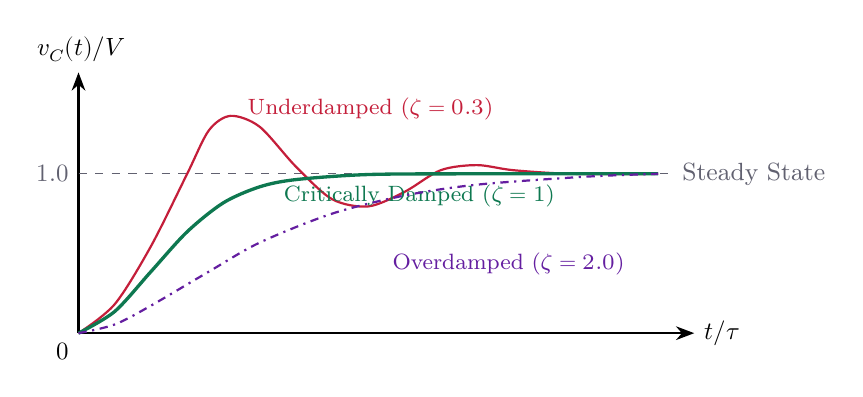
\begin{tikzpicture}[scale=0.92, every node/.style={font=\small}]
  % Axes
  \draw[-Stealth, thick] (0,0) -- (8.5,0) node[right] {$t / \tau$};
  \draw[-Stealth, thick] (0,0) -- (0,3.6) node[above] {$v_C(t) / V$};

  % Steady state line
  \draw[dashed, color=mydark!70] (0,2.2) node[left] {$1.0$} -- (8.2,2.2) node[right] {Steady State};

  % Underdamped Curve (oscillatory overshoot)
  \draw[thick, color=myred, smooth] plot coordinates {
    (0,0) (0.5,0.4) (1.0,1.2) (1.5,2.2) (1.8,2.8) (2.1,3.0) (2.5,2.85) (3.0,2.3)
    (3.5,1.85) (4.0,1.75) (4.5,1.95) (5.0,2.25) (5.5,2.32) (6.0,2.25) (6.8,2.2) (8.0,2.2)
  };
  \node[color=myred, font=\footnotesize, right] at (2.2, 3.1) {Underdamped ($\zeta = 0.3$)};

  % Critically Damped Curve (fastest rise without overshoot)
  \draw[very thick, color=mygreen, smooth] plot coordinates {
    (0,0) (0.5,0.3) (1.0,0.85) (1.5,1.4) (2.0,1.8) (2.5,2.02) (3.0,2.12) (4.0,2.19) (5.5,2.2) (8.0,2.2)
  };
  \node[color=mygreen, font=\footnotesize, above right] at (2.7, 1.6) {Critically Damped ($\zeta = 1$)};

  % Overdamped Curve (sluggish)
  \draw[thick, color=mypurple, dashdotted, smooth] plot coordinates {
    (0,0) (0.5,0.12) (1.0,0.38) (1.8,0.85) (2.5,1.25) (3.5,1.65) (4.5,1.9) (5.5,2.05) (7.0,2.16) (8.0,2.2)
  };
  \node[color=mypurple, font=\footnotesize, below right] at (4.2, 1.25) {Overdamped ($\zeta = 2.0$)};

  % Grid ticks
  \draw (0,0) node[below left] {$0$};
\end{tikzpicture}
\end{center}
\end{tcolorbox}

\subsection{Dual Parallel RLC Network}

In a parallel RLC circuit excited by an independent current step $I\,u(t)$, the dual nodal formulation gives:
\begin{equation}
  \frac{v(t)}{R} + \frac{1}{L}\int_0^t v(\tau)\,d\tau + C\,\frac{dv(t)}{dt} = I
\end{equation}
The characteristic equation and parameters are:
\begin{equation}
  s^2 + \frac{1}{RC}s + \frac{1}{LC} = 0 \implies \alpha = \frac{1}{2RC}, \quad \omega_0 = \frac{1}{\sqrt{LC}}, \quad \zeta = \frac{1}{2R}\sqrt{\frac{L}{C}}
\end{equation}

\newpage
% ===============================================================================
% MANDATORY QUICK REVISION PAGE
% ===============================================================================
\begin{center}
  {\large\bfseries\color{myred} Quick Revision --- Module 3}\\[2pt]
  {\small\color{mydark} Laplace Transforms, Network Transients and Initial Conditions $|$ EC304}
\end{center}
\noindent{\color{myred}\rule{\linewidth}{1.0pt}}
\vspace{2pt}

\begin{tcolorbox}[formulabox, top=5pt, bottom=5pt, title={\textbf{Key Formulas and Network Relations at a Glance}}]
\renewcommand{\arraystretch}{1.20}
\begin{tabularx}{\linewidth}{B{5.0cm} X}
Unilateral Laplace Transform & $F(s) = \int_{0^-}^\infty f(t)\,e^{-st}\,dt, \quad s = \sigma + j\omega$ \\[2pt]
Time Derivative Transform & $\mathcal{L}\{f'(t)\} = sF(s) - f(0^-), \quad \mathcal{L}\{f''(t)\} = s^2F(s) - s f(0^-) - f'(0^-)$ \\[2pt]
Time Shifting Property & $\mathcal{L}\{f(t - t_0)u(t - t_0)\} = e^{-s t_0} F(s) \quad (t_0 \ge 0)$ \\[2pt]
Final Value Theorem & $\lim_{t \to \infty} f(t) = \lim_{s \to 0} s F(s) \quad (\text{poles in open LHP})$ \\[2pt]
Inductor $s$-Domain Model & $V_L(s) = sL I_L(s) - L i_L(0^-) \iff I_L(s) = \frac{V_L(s)}{sL} + \frac{i_L(0^-)}{s}$ \\[2pt]
Capacitor $s$-Domain Model & $V_C(s) = \frac{I_C(s)}{sC} + \frac{v_C(0^-)}{s} \iff I_C(s) = sC V_C(s) - C v_C(0^-)$ \\[2pt]
First-Order Step Response & $x(t) = x(\infty) + [x(0^+) - x(\infty)]e^{-t/\tau}, \quad \tau_{RL} = \frac{L}{R}, \; \tau_{RC} = RC$ \\[2pt]
Series RLC Damping Parameters & $\alpha = \frac{R}{2L}, \quad \omega_0 = \frac{1}{\sqrt{LC}}, \quad \zeta = \frac{\alpha}{\omega_0} = \frac{R}{2}\sqrt{\frac{C}{L}}$ \\[2pt]
Damped Frequency & $\omega_d = \sqrt{\omega_0^2 - \alpha^2} = \omega_0\sqrt{1 - \zeta^2} \quad (\text{for } \zeta < 1)$ \\[2pt]
\end{tabularx}
\end{tcolorbox}

\begin{tcolorbox}[defbox, top=5pt, bottom=5pt, title={\textbf{One-Line Definitions}}]
\begin{itemize}[leftmargin=*, itemsep=1.0pt, topsep=0pt]
  \item \textbf{Singularity Function:} A function exhibiting discontinuities in its value or its higher-order time derivatives.
  \item \textbf{Unit Impulse $\delta(t)$:} A generalized function of infinite height, zero width, and unit integral area at $t=0$.
  \item \textbf{Lower Limit $0^-$:} The instant immediately prior to switching, capturing jump discontinuities and initial states.
  \item \textbf{Zero-Input Response (ZIR):} System response produced solely by initial stored energy with external sources zeroed.
  \item \textbf{Zero-State Response (ZSR):} System response produced solely by applied excitations with zero initial stored energy.
  \item \textbf{Time Constant ($\tau$):} Time required for a first-order transient response to decay to $36.8\%$ ($1/e$) of initial value.
  \item \textbf{Neper Frequency ($\alpha$):} Exponential damping attenuation factor governing the rate of response decay.
  \item \textbf{Undamped Resonant Frequency ($\omega_0$):} Natural oscillation frequency of an LC circuit in the absence of resistance.
  \item \textbf{Damping Ratio ($\zeta$):} Dimensionless ratio $\alpha/\omega_0$ determining whether a second-order circuit oscillates.
  \item \textbf{Critically Damped Circuit:} Second-order circuit with $\zeta=1$ returning to steady state in minimum non-oscillatory time.
\end{itemize}
\end{tcolorbox}

\begin{tcolorbox}[exambox, title={\textbf{Frequently Asked / Viva Questions}}]
\begin{enumerate}[topsep=0pt, label=\textbf{Q\arabic*.}, itemsep=4pt]
  \item \Q{Why cannot inductor current change instantaneously in a finite circuit?}
  Stored magnetic energy is $W = \frac{1}{2}L i_L^2$. An instantaneous change requires infinite power ($P = \frac{dW}{dt} \to \infty$) and infinite voltage ($v_L = L \frac{di}{dt} \to \infty$), which is impossible with finite sources. Hence, $i_L(0^+) = i_L(0^-)$.

  \item \Q{Why does an uncharged capacitor act as a short circuit at $t = 0^+$?}
  Since $v_C(0^+) = v_C(0^-) = 0\text{ V}$, the terminal voltage is zero immediately after switching while current flows freely. An element supporting finite current with zero voltage drop behaves identically to an ideal short circuit.

  \item \Q{Explain the physical necessity of the lower limit $0^-$ in unilateral Laplace transforms.}
  The $0^-$ limit captures Dirac delta impulses $\delta(t)$ acting at $t=0$ and accounts for pre-switching initial conditions ($i_L(0^-), v_C(0^-)$). A lower limit of $0^+$ would omit impulses occurring at the switching origin.

  \item \Q{State the validity condition for applying the Final Value Theorem.}
  $\lim_{t \to \infty} f(t) = \lim_{s \to 0} sF(s)$ is valid strictly if all poles of $sF(s)$ lie in the open left-half $s$-plane. If poles lie on the imaginary axis (e.g. sustained sinusoids) or in the right-half plane, FVT produces incorrect results.

  \item \Q{Distinguish between natural and forced responses in circuit transients.}
  The natural (transient) response depends solely on circuit storage elements ($R, L, C$) and decays to zero. The forced (steady-state) response is sustained by external driving sources and mirrors their functional form.

  \item \Q{Under what switching condition is an AC RL circuit completely transient-free?}
  In an RL circuit excited by $v(t) = V_m\sin(\omega t + \theta)$, transient-free operation occurs when switching at $\theta - \phi = 0$ or $\pi$ (where $\phi = \tan^{-1}\frac{\omega L}{R}$), matching prospective steady-state current to the initial zero current.

  \item \Q{How does the Norton $s$-domain model of an inductor differ from its Thevenin form?}
  The Thevenin form consists of an impedance $sL$ in series with an opposing voltage source $L i_L(0^-)$. The Norton form comprises an admittance $\frac{1}{sL}$ in parallel with a current source $\frac{i_L(0^-)}{s}$ pointing in the direction of $i_L$.

  \item \Q{Define damping ratio $\zeta$ and give its formulas for series and parallel RLC circuits.}
  $\zeta = \alpha / \omega_0$. For series RLC: $\zeta = \frac{R}{2}\sqrt{\frac{C}{L}}$. For parallel RLC: $\zeta = \frac{1}{2R}\sqrt{\frac{L}{C}}$.

  \item \Q{Why is critical damping ($\zeta = 1$) preferred in analog meters and galvanometers?}
  Critical damping ensures the pointer reaches its steady deflection in the shortest possible time without oscillatory overshoot or sluggish delay, enabling fast, accurate readings.

  \item \Q{What is the circuit significance of the unit doublet $\delta'(t)$?}
  The unit doublet represents $\frac{d\delta}{dt}$. In circuits, it arises from impulsive current injection across inductors or impulse voltage across capacitors, abruptly altering state variables at $t=0$.
\end{enumerate}
\end{tcolorbox}

\begin{tcolorbox}[tikzbox, title={\textbf{Summary Matrix: Comprehensive Comparison of First- and Second-Order Transients}}]
\par\vspace{3pt}\noindent
\begingroup
\setlength{\tabcolsep}{4.0pt}
\setlength{\extrarowheight}{2.0pt}
\renewcommand{\arraystretch}{1.22}
\begin{tabularx}{\linewidth}{|B{2.3cm}|B{3.0cm}|B{3.2cm}|Y|}
\hline
\textbf{Circuit Type} & \textbf{Time Const. / Damping} & \textbf{Roots} & \textbf{Transient Response Nature} \\
\hline
Series RL & $\tau = \dfrac{L}{R}$ & $s = -\dfrac{R}{L}$ & Monotonic exponential rise/decay; no oscillation. \\
\hline
Series RC & $\tau = RC$ & $s = -\dfrac{1}{RC}$ & Monotonic exponential voltage change; current step at $t=0^+$. \\
\hline
Series RLC Overdamped & $\alpha = \dfrac{R}{2L} > \omega_0$,\\[2pt]$\zeta > 1$ & $s_{1,2} = -\alpha \pm \sqrt{\alpha^2 - \omega_0^2}$ & Sum of two decaying exponentials; sluggish, non-oscillatory. \\
\hline
Series RLC Critically Damped & $\alpha = \omega_0$,\\[2pt]$\zeta = 1$ & $s_1 = s_2 = -\alpha$ & Rapid monotonic return to equilibrium without overshoot ($(A_1+A_2 t)e^{-\alpha t}$). \\
\hline
Series RLC Underdamped & $\alpha < \omega_0$,\\[2pt]$\zeta < 1$ & $s_{1,2} = -\alpha \pm j\omega_d$ & Damped sinusoidal oscillations with decaying envelope $e^{-\alpha t}$. \\
\hline
Parallel RLC & $\alpha = \dfrac{1}{2RC}$,\\[2pt]$\zeta = \dfrac{1}{2R}\sqrt{\dfrac{L}{C}}$ & $s_{1,2} = -\alpha \pm \sqrt{\alpha^2 - \omega_0^2}$ & Dual of series RLC; higher $R$ produces lower damping (oscillatory). \\
\hline
\end{tabularx}
\endgroup
\end{tcolorbox}


% -- Module 4 -----------------------------------------------------------------
\modulestart{4}{Complex Frequency and Network Functions}

\section{Complex Frequency and Network Functions}

The concept of complex frequency generalizes real sinusoidal and exponential signals into a unified mathematical framework. It forms the foundation for characterizing linear time-invariant (LTI) networks in the complex frequency $s$-plane.

\subsection{Concept of Complex Frequency}

\begin{tcolorbox}[defbox, title={\textbf{Definition of Complex Frequency}}]
A generalized damped sinusoidal signal is expressed as:
\begin{equation}
  f(t) = A\,e^{\sigma t}\,\cos(\omega t + \theta) = \text{Re}\left\{ A\,e^{j\theta}\,e^{(\sigma + j\omega)t} \right\} = \text{Re}\left\{ \mathbf{F}\,e^{st} \right\}
\end{equation}
The parameter $s = \sigma + j\omega$ is the \textbf{complex frequency} (measured in $\text{s}^{-1}$ or complex nepers/radians per second):
\begin{itemize}[leftmargin=*]
  \item $\sigma = \text{Re}(s)$ is the \textbf{Neper frequency} (damping or growth rate in Np/s).
  \item $\omega = \text{Im}(s)$ is the \textbf{radian angular frequency} (oscillation rate in rad/s).
\end{itemize}
\end{tcolorbox}

\begin{tcolorbox}[formulabox, title={\textbf{Special Cases of the Complex Frequency Variable $s = \sigma + j\omega$}}]
\begin{enumerate}[leftmargin=*]
  \item $\sigma = 0, \omega = 0 \implies s = 0$: Constant DC signal ($f(t) = A$).
  \item $\sigma \ne 0, \omega = 0 \implies s = \sigma$: Pure exponential signal ($e^{\sigma t}$; decaying if $\sigma < 0$, growing if $\sigma > 0$).
  \item $\sigma = 0, \omega \ne 0 \implies s = j\omega$: Undamped steady-state sinusoidal signal ($A\cos(\omega t)$).
  \item $\sigma < 0, \omega \ne 0$: Damped sinusoidal signal (exponentially decaying oscillatory transient).
  \item $\sigma > 0, \omega \ne 0$: Growing sinusoidal signal (unstable active system).
\end{enumerate}
\end{tcolorbox}

\subsection{Definition and Classification of Network Functions}

\begin{tcolorbox}[defbox, title={\textbf{Network Function Definition}}]
For a linear, lumped, time-invariant network with all initial conditions set to zero (relaxed state), a \textbf{Network Function} $H(s)$ is defined as the ratio of the Laplace transform of the output response $R(s)$ to the Laplace transform of the input excitation $E(s)$:
\begin{equation}
  H(s) = \frac{R(s)}{E(s)} \iff R(s) = H(s) \cdot E(s)
\end{equation}
\end{tcolorbox}

Network functions are broadly classified into two categories:
\begin{enumerate}[leftmargin=*]
  \item \textbf{Driving-Point Immittance Functions:} Excitation and response are measured at the \textbf{same port}:
  \begin{itemize}
    \item \textit{Driving-point impedance:} $Z_{in}(s) = \dfrac{V_1(s)}{I_1(s)}$
    \item \textit{Driving-point admittance:} $Y_{in}(s) = \dfrac{I_1(s)}{V_1(s)} = \dfrac{1}{Z_{in}(s)}$
  \end{itemize}
  \item \textbf{Transfer Functions:} Excitation and response are measured at \textbf{different ports}:
  \begin{itemize}
    \item \textit{Voltage Transfer Function (Gain):} $G_{21}(s) = \dfrac{V_2(s)}{V_1(s)}$
    \item \textit{Current Transfer Function (Gain):} $\alpha_{21}(s) = \dfrac{I_2(s)}{I_1(s)}$
    \item \textit{Transfer Impedance:} $Z_{21}(s) = \dfrac{V_2(s)}{I_1(s)}$
    \item \textit{Transfer Admittance:} $Y_{21}(s) = \dfrac{I_2(s)}{V_1(s)}$
  \end{itemize}
\end{enumerate}

% ===============================================================================
% SECTION 2: POLES AND ZEROS OF NETWORK FUNCTIONS
% ===============================================================================
\section{Poles and Zeros of Immittance Functions and their Properties}

Any network function of a lumped LTI circuit can be expressed as a rational function of $s$ with real coefficients:
\begin{equation}
  H(s) = \frac{N(s)}{D(s)} = \frac{a_m s^m + a_{m-1} s^{m-1} + \cdots + a_1 s + a_0}{b_n s^n + b_{n-1} s^{n-1} + \cdots + b_1 s + b_0} = K \frac{\prod_{i=1}^m (s - z_i)}{\prod_{k=1}^n (s - p_k)}
\end{equation}

\subsection{Definitions of Poles and Zeros}

\begin{tcolorbox}[defbox, title={\textbf{Poles and Zeros}}]
\begin{itemize}[leftmargin=*]
  \item \textbf{Zeros ($z_i$):} The values of complex frequency $s$ for which $H(s) = 0$ (roots of the numerator $N(s) = 0$). At a transmission zero, the network completely suppresses the input signal.
  \item \textbf{Poles ($p_k$):} The values of complex frequency $s$ for which $H(s) \to \infty$ (roots of the denominator $D(s) = 0$). Poles define the natural frequencies (modes) and determine stability.
  \item \textbf{Critical Frequencies at Infinity:} If $n > m$, $H(s)$ has $(n - m)$ zeros at $s = \infty$. If $m > n$, $H(s)$ has $(m - n)$ poles at $s = \infty$. The total number of zeros equals the total number of poles in the extended complex plane.
\end{itemize}
\end{tcolorbox}

\subsection{Properties of Driving-Point Immittances (Positive Real Functions)}

For any passive, bilateral electrical network without internal active sources, the driving-point immittance $Z(s)$ or $Y(s)$ must be a \textbf{Positive Real (PR) Function} (Brune's condition):
\begin{equation}
  \text{Re}\{Z(s)\} \ge 0 \quad \text{whenever} \quad \text{Re}(s) \ge 0
\end{equation}

\begin{tcolorbox}[formulabox, title={\textbf{Necessary and Sufficient Properties of Passive Immittance Functions}}]
\begin{enumerate}[leftmargin=*]
  \item \textbf{Hurwitz Denominator and Numerator:} All poles and zeros of $Z(s)$ must lie in the left half of the $s$-plane ($\text{Re}(s) \le 0$). They cannot reside in the open right-half plane (RHP).
  \item \textbf{Imaginary Axis Poles and Zeros:} Any poles and zeros located on the $j\omega$-axis must be \textbf{simple} (multiplicity of 1). Multiple poles on the $j\omega$-axis are strictly forbidden because they generate unbounded polynomial-exponential terms ($t\sin\omega t$).
  \item \textbf{Residue Condition:} The residues of $Z(s)$ at simple poles on the $j\omega$-axis must be \textbf{real and strictly positive}.
  \item \textbf{Degree Constraint:} The degrees of the numerator polynomial $N(s)$ and denominator polynomial $D(s)$ can differ at most by $1$: $|m - n| \le 1$.
  \item \textbf{Lowest Degree Constraint:} The lowest power of $s$ in $N(s)$ and $D(s)$ can differ at most by $1$.
  \item \textbf{Foster Alternation Law (LC Immittance):} For purely reactive lossless LC networks, all poles and zeros lie exclusively on the $j\omega$-axis, are simple, and must strictly \textbf{interlace (alternate)}:
  \begin{equation}
    0 \le \omega_{z1} < \omega_{p1} < \omega_{z2} < \omega_{p2} < \cdots
  \end{equation}
  Furthermore, the slope of reactance with respect to frequency is strictly positive: $\frac{dX(\omega)}{d\omega} > 0$.
\end{enumerate}
\end{tcolorbox}

% ===============================================================================
% SECTION 3: FREQUENCY RESPONSE FROM POLE-ZERO LOCATIONS
% ===============================================================================
\section{Sinusoidal Steady-State Response from Pole-Zero Locations}

The steady-state frequency response $H(j\omega)$ of any network function can be evaluated directly by geometric inspection of its pole-zero constellation in the $s$-plane.

\subsection{Geometric Vector Formulation}

Evaluating $H(s)$ on the imaginary axis $s = j\omega$:
\begin{equation}
  H(j\omega) = K \frac{(j\omega - z_1)(j\omega - z_2)\cdots(j\omega - z_m)}{(j\omega - p_1)(j\omega - p_2)\cdots(j\omega - p_n)}
\end{equation}
Each term $(j\omega - z_i)$ represents a directed complex vector in the $s$-plane from the zero $z_i$ to the test frequency point $s = j\omega$:
\begin{equation}
  (j\omega - z_i) = M_i\,e^{j\psi_i}, \quad \text{where } M_i = |j\omega - z_i|, \quad \psi_i = \angle(j\omega - z_i)
\end{equation}
Similarly, each term $(j\omega - p_k)$ represents a vector from the pole $p_k$ to the test point $j\omega$:
\begin{equation}
  (j\omega - p_k) = N_k\,e^{j\theta_k}, \quad \text{where } N_k = |j\omega - p_k|, \quad \theta_k = \angle(j\omega - p_k)
\end{equation}

\begin{tcolorbox}[formulabox, title={\textbf{Magnitude and Phase Computation via Pole-Zero Geometry}}]
\begin{align}
  |H(j\omega)| &= |K| \cdot \frac{M_1 M_2 \cdots M_m}{N_1 N_2 \cdots N_n} = |K| \cdot \frac{\prod (\text{distances from zeros to } j\omega)}{\prod (\text{distances from poles to } j\omega)} \\[5pt]
  \angle H(j\omega) &= \angle K + \sum_{i=1}^m \psi_i - \sum_{k=1}^n \theta_k = \angle K + \sum(\text{zero angles}) - \sum(\text{pole angles})
\end{align}
\end{tcolorbox}

\begin{tcolorbox}[tikzbox, title={\textbf{TikZ Schematic: Geometric Vector Evaluation in the Complex $s$-Plane}}]
\begin{center}
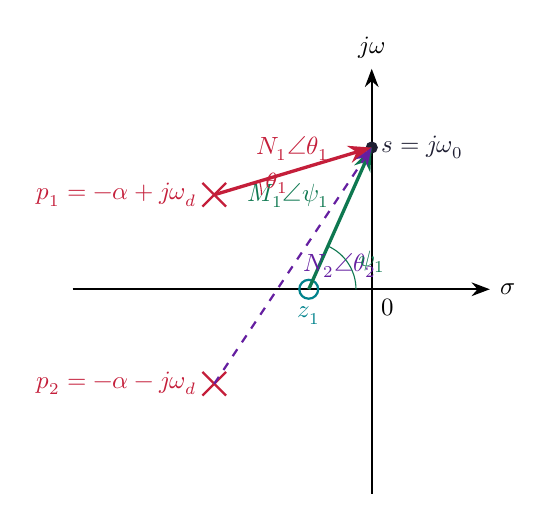
\begin{tikzpicture}[scale=1.0, every node/.style={font=\small}]
  % Axes
  \draw[-Stealth, thick] (-3.8,0) -- (1.5,0) node[right] {$\sigma$};
  \draw[-Stealth, thick] (0,-2.6) -- (0,2.8) node[above] {$j\omega$};

  % Origin
  \node[below right] at (0,0) {$0$};

  % Poles and Zeros
  \coordinate (P1) at (-2.0, 1.2);
  \coordinate (P2) at (-2.0, -1.2);
  \coordinate (Z1) at (-0.8, 0);
  \coordinate (JW) at (0, 1.8);

  % Draw Poles (X) and Zeros (O)
  \draw[thick, color=myred] ($(P1)+(-0.15,-0.15)$) -- ($(P1)+(0.15,0.15)$);
  \draw[thick, color=myred] ($(P1)+(-0.15,0.15)$) -- ($(P1)+(0.15,-0.15)$);
  \node[left=0.1cm of P1, color=myred] {$p_1 = -\alpha + j\omega_d$};

  \draw[thick, color=myred] ($(P2)+(-0.15,-0.15)$) -- ($(P2)+(0.15,0.15)$);
  \draw[thick, color=myred] ($(P2)+(-0.15,0.15)$) -- ($(P2)+(0.15,-0.15)$);
  \node[left=0.1cm of P2, color=myred] {$p_2 = -\alpha - j\omega_d$};

  \draw[thick, color=myteal] (Z1) circle (0.12);
  \node[below=0.1cm of Z1, color=myteal] {$z_1$};

  % Evaluation point on jw axis
  \filldraw[color=mydark] (JW) circle (0.07) node[right] {$s = j\omega_0$};

  % Vectors from pole/zero to jw point
  \draw[-Stealth, very thick, color=mygreen] (Z1) -- (JW) node[midway, above left] {$M_1 \angle \psi_1$};
  \draw[-Stealth, very thick, color=myred] (P1) -- (JW) node[midway, above] {$N_1 \angle \theta_1$};
  \draw[-Stealth, thick, dashed, color=mypurple] (P2) -- (JW) node[midway, right] {$N_2 \angle \theta_2$};

  % Angle arcs
  \draw[thin, color=mygreen] ($(Z1)+(0.6,0)$) arc (0:66:0.6);
  \node[color=mygreen, font=\footnotesize] at ($(Z1)+(0.8,0.35)$) {$\psi_1$};

  \draw[thin, color=myred] ($(P1)+(0.6,0)$) arc (0:17:0.6);
  \node[color=myred, font=\footnotesize] at ($(P1)+(0.8,0.15)$) {$\theta_1$};
\end{tikzpicture}
\end{center}
\end{tcolorbox}

% ===============================================================================
% SECTION 4: CONVOLUTION THEOREM IN ELECTRICAL CIRCUITS
% ===============================================================================
\section{The Convolution Theorem in Electrical Networks}

The convolution theorem establishes the fundamental mathematical bridge between time-domain input-output relationships and $s$-domain transfer function multiplication.

\subsection{Mathematical Definition and Circuit Interpretation}

\begin{tcolorbox}[defbox, title={\textbf{Time Convolution Theorem}}]
Let $h(t)$ be the \textbf{impulse response} of a relaxed LTI network (the response when excited by $x(t) = \delta(t)$). The zero-state response $y(t)$ to an arbitrary continuous excitation $x(t)$ applied at $t=0$ is given by the convolution integral:
\begin{equation}
  y(t) = x(t) * h(t) = \int_{0^-}^t x(\tau)\,h(t - \tau)\,d\tau = \int_{0^-}^t h(\tau)\,x(t - \tau)\,d\tau
\end{equation}
In the transformed frequency domain:
\begin{equation}
  \mathcal{L}\{x(t) * h(t)\} = X(s) \cdot H(s) \iff Y(s) = H(s) X(s)
\end{equation}
where $H(s) = \mathcal{L}\{h(t)\}$ is the transfer function of the network.
\end{tcolorbox}

\begin{tcolorbox}[formulabox, title={\textbf{Relation Between Impulse Response and Step Response}}]
If $s(t)$ represents the unit step response ($x(t) = u(t)$) of a linear network:
\begin{equation}
  s(t) = u(t) * h(t) = \int_{0^-}^t h(\tau)\,d\tau \iff h(t) = \frac{ds(t)}{dt}
\end{equation}
The unit impulse response is the exact time derivative of the unit step response.
\end{tcolorbox}

% ===============================================================================
% SECTION 5: TWO-PORT NETWORK PARAMETERS AND INTERCONNECTIONS
% ===============================================================================
\section{Two-Port Network Parameters and Interconnections}

A two-port network is a four-terminal electrical network having two distinct access ports: Port 1 (input port, terminals $1-1'$) and Port 2 (output port, terminals $2-2'$). Standard sign convention assumes terminal currents $I_1$ and $I_2$ enter the positive terminal of their respective ports.

\begin{tcolorbox}[tikzbox, title={\textbf{TikZ Schematic: Standard Terminal Variable Convention for a Two-Port Network}}]
\begin{center}
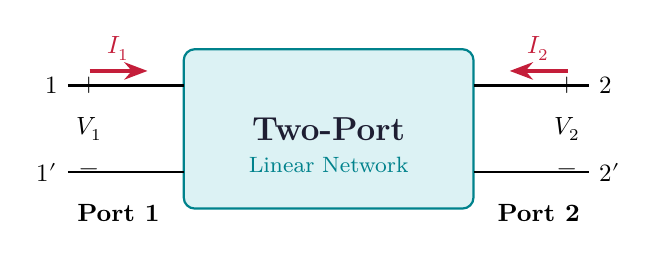
\begin{tikzpicture}[scale=0.92, every node/.style={font=\small}]
  % Two-port box
  \draw[thick, fill=hdrteal, draw=myteal, rounded corners=4pt] (2,0) rectangle (6,2.2);
  \node[font=\large\bfseries\color{mydark}] at (4,1.1) {Two-Port};
  \node[font=\footnotesize\color{myteal}] at (4,0.6) {Linear Network};

  % Port 1
  \draw[thick] (0.4,1.7) node[left] {$1$} -- (2,1.7);
  \draw[thick] (0.4,0.5) node[left] {$1'$} -- (2,0.5);
  \draw[-Stealth, very thick, color=myred] (0.7,1.9) -- (1.5,1.9) node[midway, above] {$I_1$};
  \node at (0.7, 1.7) {$+$};
  \node at (0.7, 0.5) {$-$};
  \node at (0.7, 1.1) {$V_1$};
  \node[below=0.1cm] at (1.1,0.3) {\textbf{Port 1}};

  % Port 2
  \draw[thick] (6,1.7) -- (7.6,1.7) node[right] {$2$};
  \draw[thick] (6,0.5) -- (7.6,0.5) node[right] {$2'$};
  \draw[-Stealth, very thick, color=myred] (7.3,1.9) -- (6.5,1.9) node[midway, above] {$I_2$};
  \node at (7.3, 1.7) {$+$};
  \node at (7.3, 0.5) {$-$};
  \node at (7.3, 1.1) {$V_2$};
  \node[below=0.1cm] at (6.9,0.3) {\textbf{Port 2}};
\end{tikzpicture}
\end{center}
\end{tcolorbox}

\subsection{The Six Fundamental Two-Port Parameter Sets}

\begin{tcolorbox}[defbox, title={\textbf{Definitions and Equations of Two-Port Parameter Sets}}]
\begin{enumerate}[leftmargin=*, itemsep=4pt]
  \item \textbf{Impedance ($Z$) Parameters (Open-Circuit Parameters):}
  \begin{equation}
    \begin{bmatrix} V_1 \\ V_2 \end{bmatrix} = \begin{bmatrix} z_{11} & z_{12} \\ z_{21} & z_{22} \end{bmatrix} \begin{bmatrix} I_1 \\ I_2 \end{bmatrix} \implies \begin{aligned} V_1 &= z_{11} I_1 + z_{12} I_2 \\ V_2 &= z_{21} I_1 + z_{22} I_2 \end{aligned}
  \end{equation}
  $z_{11} = \left.\frac{V_1}{I_1}\right|_{I_2=0}$ (input impedance), $z_{12} = \left.\frac{V_1}{I_2}\right|_{I_1=0}$ (reverse transfer impedance),\\
  $z_{21} = \left.\frac{V_2}{I_1}\right|_{I_2=0}$ (forward transfer impedance), $z_{22} = \left.\frac{V_2}{I_2}\right|_{I_1=0}$ (output impedance).

  \item \textbf{Admittance ($Y$) Parameters (Short-Circuit Parameters):}
  \begin{equation}
    \begin{bmatrix} I_1 \\ I_2 \end{bmatrix} = \begin{bmatrix} y_{11} & y_{12} \\ y_{21} & y_{22} \end{bmatrix} \begin{bmatrix} V_1 \\ V_2 \end{bmatrix} \implies \begin{aligned} I_1 &= y_{11} V_1 + y_{12} V_2 \\ I_2 &= y_{21} V_1 + y_{22} V_2 \end{aligned}
  \end{equation}
  $[Y] = [Z]^{-1} \implies y_{11} = \frac{z_{22}}{\Delta z}, \quad y_{12} = -\frac{z_{12}}{\Delta z}, \quad y_{21} = -\frac{z_{21}}{\Delta z}, \quad y_{22} = \frac{z_{11}}{\Delta z}$.

  \item \textbf{Transmission ($ABCD$) Parameters (Cascade / Chain Parameters):}
  Relates input terminal variables to output terminal variables under reverse current load convention:
  \begin{equation}
    \begin{bmatrix} V_1 \\ I_1 \end{bmatrix} = \begin{bmatrix} A & B \\ C & D \end{bmatrix} \begin{bmatrix} V_2 \\ -I_2 \end{bmatrix} \implies \begin{aligned} V_1 &= A V_2 - B I_2 \\ I_1 &= C V_2 - D I_2 \end{aligned}
  \end{equation}
  $A = \left.\frac{V_1}{V_2}\right|_{I_2=0}$ (reverse voltage ratio), $B = \left.\frac{V_1}{-I_2}\right|_{V_2=0}$ (transfer impedance),\\
  $C = \left.\frac{I_1}{V_2}\right|_{I_2=0}$ (transfer admittance), $D = \left.\frac{I_1}{-I_2}\right|_{V_2=0}$ (reverse current ratio).

  \item \textbf{Hybrid ($h$) Parameters:}
  Used extensively in small-signal bipolar transistor modeling:
  \begin{equation}
    \begin{bmatrix} V_1 \\ I_2 \end{bmatrix} = \begin{bmatrix} h_{11} & h_{12} \\ h_{21} & h_{22} \end{bmatrix} \begin{bmatrix} I_1 \\ V_2 \end{bmatrix} \implies \begin{aligned} V_1 &= h_{11} I_1 + h_{12} V_2 \\ I_2 &= h_{21} I_1 + h_{22} V_2 \end{aligned}
  \end{equation}

  \item \textbf{Inverse Hybrid ($g$) Parameters:}
  Used in field-effect transistor modeling:
  \begin{equation}
    \begin{bmatrix} I_1 \\ V_2 \end{bmatrix} = \begin{bmatrix} g_{11} & g_{12} \\ g_{21} & g_{22} \end{bmatrix} \begin{bmatrix} V_1 \\ I_2 \end{bmatrix} \implies \begin{aligned} I_1 &= g_{11} V_1 + g_{12} I_2 \\ V_2 &= g_{21} V_1 + g_{22} I_2 \end{aligned}
  \end{equation}
\end{enumerate}
\end{tcolorbox}

\subsection{Reciprocity and Symmetry Conditions}

\par\vspace{6pt}\noindent
\begingroup
\setlength{\tabcolsep}{5pt}
\setlength{\extrarowheight}{3pt}
\renewcommand{\arraystretch}{1.38}
\begin{tabularx}{\linewidth}{|B{3.5cm}|B{4.0cm}|Y|}
\hline
\multicolumn{1}{|c|}{\textbf{Parameter Set}} & \multicolumn{1}{c|}{\textbf{Reciprocity Condition}} & \multicolumn{1}{c|}{\textbf{Symmetry Condition}} \\
\hline
Impedance ($Z$) & $z_{12} = z_{21}$ & $z_{11} = z_{22}$ \\
\hline
Admittance ($Y$) & $y_{12} = y_{21}$ & $y_{11} = y_{22}$ \\
\hline
Transmission ($ABCD$) & $AD - BC = 1$ & $A = D$ \\
\hline
Hybrid ($h$) & $h_{12} = -h_{21}$ & $\Delta h = h_{11} h_{22} - h_{12} h_{21} = 1$ \\
\hline
Inverse Hybrid ($g$) & $g_{12} = -g_{21}$ & $\Delta g = g_{11} g_{22} - g_{12} g_{21} = 1$ \\
\hline
\end{tabularx}
\endgroup
\vspace{12pt}

\subsection{Interconnections of Two-Port Networks}

When two-port networks $N_A$ and $N_B$ are interconnected, their overall parameter matrices combine algebraically:

\begin{tcolorbox}[defbox, title={\textbf{Combination Rules for Interconnected Two-Ports}}]
\begin{enumerate}[leftmargin=*]
  \item \textbf{Series-Series Connection:} Input ports connected in series, output ports in series:
  \begin{equation}
    [Z] = [Z_A] + [Z_B]
  \end{equation}
  \item \textbf{Parallel-Parallel Connection:} Input ports in parallel, output ports in parallel:
  \begin{equation}
    [Y] = [Y_A] + [Y_B]
  \end{equation}
  \item \textbf{Cascade (Tandem) Connection:} Output of $N_A$ connected to input of $N_B$:
  \begin{equation}
    [T] = [T_A] \times [T_B] = \begin{bmatrix} A_A & B_A \\ C_A & D_A \end{bmatrix} \begin{bmatrix} A_B & B_B \\ C_B & D_B \end{bmatrix}
  \end{equation}
  \item \textbf{Series-Parallel Connection:} Input ports in series, output ports in parallel:
  \begin{equation}
    [h] = [h_A] + [h_B]
  \end{equation}
\end{enumerate}
\textbf{Brune's Test for Validity:} When combining two-port networks in series or parallel, circulating loop currents between the two networks can violate the fundamental port condition ($i_{\text{in}} = i_{\text{return}}$). Brune's test confirms validity: if the terminal voltage across the interconnection points is zero before connection, the matrices can be added directly without ideal isolation transformers.
\end{tcolorbox}

% ===============================================================================
% SECTION 6: SERIES AND PARALLEL RESONANCE
% ===============================================================================
\section{Behaviors of Series and Parallel Resonant Circuits}

Resonance is a phenomenon in reactive circuits where inductive and capacitive reactances cancel each other out at a specific frequency, causing the total input impedance to become purely real and the circuit power factor to equal unity ($\cos\phi = 1$).

\subsection{Series Resonance}

Consider an RLC branch connected in series across an AC source $\mathbf{V}$. The total complex impedance is:
\begin{equation}
  \mathbf{Z}(j\omega) = R + j\left(\omega L - \frac{1}{\omega C}\right)
\end{equation}

\begin{tcolorbox}[formulabox, title={\textbf{Series Resonance Equations}}]
\begin{enumerate}[leftmargin=*]
  \item \textbf{Resonance Condition:} Net reactance is identically zero:
  \begin{equation}
    X_L = X_C \implies \omega_0 L = \frac{1}{\omega_0 C} \implies \omega_0 = \frac{1}{\sqrt{LC}} \text{ rad/s}, \quad f_0 = \frac{1}{2\pi\sqrt{LC}} \text{ Hz}
  \end{equation}
  \item \textbf{Impedance at Resonance:} Minimum and purely resistive:
  \begin{equation}
    \mathbf{Z}(j\omega_0) = Z_{\min} = R \implies \mathbf{I}_0 = \frac{\mathbf{V}}{R} \quad (\text{Maximum Current})
  \end{equation}
  \item \textbf{Quality Factor ($Q$):} Defined as $2\pi \times \frac{\text{Maximum Energy Stored}}{\text{Energy Dissipated per Cycle}}$:
  \begin{equation}
    Q_0 = \frac{\omega_0 L}{R} = \frac{1}{\omega_0 C R} = \frac{1}{R}\sqrt{\frac{L}{C}}
  \end{equation}
  \item \textbf{Voltage Magnification:} Reactive voltages across $L$ and $C$ can far exceed source voltage:
  \begin{equation}
    V_L(j\omega_0) = V_C(j\omega_0) = Q_0 \cdot V
  \end{equation}
  \item \textbf{Half-Power Frequencies and Bandwidth ($BW$):}
  The frequencies $\omega_1$ (lower) and $\omega_2$ (upper) where current magnitude drops to $I_0/\sqrt{2}$ ($70.7\%$) and dissipated active power drops to $P_{\max}/2$:
  \begin{equation}
    \omega_{1,2} = \mp \frac{R}{2L} + \sqrt{\left(\frac{R}{2L}\right)^2 + \frac{1}{LC}} \implies BW = \Delta\omega = \omega_2 - \omega_1 = \frac{R}{L} = \frac{\omega_0}{Q_0}
  \end{equation}
  Geometric center frequency relation: $\omega_0 = \sqrt{\omega_1 \omega_2}$. For high-$Q$ circuits ($Q \ge 10$), arithmetic symmetry holds: $\omega_1 \approx \omega_0 - \frac{BW}{2}, \quad \omega_2 \approx \omega_0 + \frac{BW}{2}$.
\end{enumerate}
\end{tcolorbox}

\subsection{Parallel Resonance (Practical Tank Circuit)}

A practical inductor possesses winding resistance $R_L$. The practical parallel tank consists of a coil ($R_L$ in series with $L$) connected in parallel with an ideal capacitor $C$.
\begin{equation}
  \mathbf{Y} = \frac{1}{R_L + j\omega L} + j\omega C = \frac{R_L - j\omega L}{R_L^2 + \omega^2 L^2} + j\omega C = \frac{R_L}{R_L^2 + \omega^2 L^2} + j\left(\omega C - \frac{\omega L}{R_L^2 + \omega^2 L^2}\right)
\end{equation}

\begin{tcolorbox}[defbox, title={\textbf{Practical Tank Circuit Resonance Conditions}}]
\begin{enumerate}[leftmargin=*]
  \item \textbf{Unity Power Factor Resonant Frequency $\omega_r$:} Setting net susceptance to zero:
  \begin{equation}
    \omega_r C = \frac{\omega_r L}{R_L^2 + \omega_r^2 L^2} \implies \omega_r = \sqrt{\frac{1}{LC} - \frac{R_L^2}{L^2}} = \omega_0\sqrt{1 - \frac{R_L^2 C}{L}}
  \end{equation}
  Physical condition for parallel resonance to occur: $\dfrac{L}{C} > R_L^2$.
  \item \textbf{Dynamic Impedance ($Z_d$):} At resonance, the circuit exhibits \textbf{maximum impedance} (anti-resonance):
  \begin{equation}
    Z_d = \frac{1}{Y_{\min}} = \frac{R_L^2 + \omega_r^2 L^2}{R_L} = \frac{L}{C R_L} \quad (\Omega)
  \end{equation}
  Total line current is minimum: $I_{\min} = \frac{V}{Z_d} = \frac{V C R_L}{L}$.
  \item \textbf{Current Magnification:} Circulating loop current between coil and capacitor is $Q$ times line current:
  \begin{equation}
    I_{\text{circ}} \approx Q \cdot I_{\text{line}}, \quad \text{where } Q = \frac{\omega_r L}{R_L}
  \end{equation}
\end{enumerate}
\end{tcolorbox}

% ===============================================================================
% SECTION 7: INTRODUCTION TO PASSIVE FILTERS
% ===============================================================================
\section{Introduction to Passive Electric Filters}

An electric filter is a frequency-selective two-port network designed to transmit signals within specified frequency bands (\textbf{pass bands}) with minimal attenuation, while significantly attenuating signals outside those bands (\textbf{attenuation / stop bands}).

\subsection{Propagation Characteristics and Cut-Off Frequency}

For a symmetrical reactive network terminated in its characteristic impedance $Z_0$:
\begin{equation}
  \frac{\mathbf{V}_1}{\mathbf{V}_2} = \frac{\mathbf{I}_1}{\mathbf{I}_2} = e^\gamma = e^{\alpha + j\beta} \implies \gamma = \alpha + j\beta
\end{equation}
where $\gamma$ is the complex propagation constant, $\alpha$ is the attenuation constant (in Nepers), and $\beta$ is the phase shift constant (in radians).
\begin{itemize}[leftmargin=*]
  \item \textbf{Pass Band:} $\alpha = 0$, signals pass with zero attenuation ($|\mathbf{V}_2/\mathbf{V}_1| = 1$), experiencing only a phase delay $\beta$.
  \item \textbf{Stop Band:} $\alpha > 0$, signal amplitude decays exponentially.
  \item \textbf{Cut-Off Frequency ($f_c$):} The boundary frequency demarcating the pass band from the stop band, defined where $\alpha = 0$ begins to increase.
\end{itemize}

\subsection{Constant-$k$ Prototype Filter Sections}

A symmetrical ladder network has series impedance $Z_1$ and shunt impedance $Z_2$. It is termed a \textbf{constant-$k$ filter} if:
\begin{equation}
  Z_1 \cdot Z_2 = k^2 = R_0^2 \quad (\text{independent of frequency})
\end{equation}
where $R_0 = \sqrt{L/C}$ is the nominal design characteristic resistance.

\par\vspace{6pt}\noindent
\begingroup
\setlength{\tabcolsep}{4.0pt}
\setlength{\extrarowheight}{2.5pt}
\renewcommand{\arraystretch}{1.25}
\begin{tabularx}{\linewidth}{|B{2.5cm}|B{3.0cm}|B{3.0cm}|Y|}
\hline
\textbf{Filter Type} & \textbf{Series Arm $Z_1$} & \textbf{Shunt Arm $Z_2$} & \textbf{Cut-off \& Design Formulas} \\
\hline
Low-Pass (LPF) & Inductor $L$ ($j\omega L$) & Capacitor $C$ ($\frac{1}{j\omega C}$) & $f_c = \frac{1}{\pi\sqrt{LC}}$,\\[2pt]$L = \frac{R_0}{\pi f_c}, \quad C = \frac{1}{\pi f_c R_0}$ \\
\hline
High-Pass (HPF) & Capacitor $C$ ($\frac{1}{j\omega C}$) & Inductor $L$ ($j\omega L$) & $f_c = \frac{1}{4\pi\sqrt{LC}}$,\\[2pt]$L = \frac{R_0}{4\pi f_c}, \quad C = \frac{1}{4\pi f_c R_0}$ \\
\hline
Band-Pass (BPF) & Series resonant ($L_1, C_1$) & Parallel resonant ($L_2, C_2$) & $f_0 = \sqrt{f_1 f_2}, \quad BW = f_2 - f_1$ \\
\hline
Band-Reject (BRF) & Parallel resonant ($L_1, C_1$) & Series resonant ($L_2, C_2$) & Stops band between $f_1$ and $f_2$; passes DC and high AC. \\
\hline
\end{tabularx}
\endgroup
\vspace{12pt}

\begin{tcolorbox}[masonbox, title={\textbf{Limitations of Constant-$k$ Filters and Evolution to $m$-Derived Filters}}]
\begin{enumerate}[leftmargin=*]
  \item \textbf{Gradual Attenuation Rise:} The attenuation $\alpha$ of a constant-$k$ filter rises slowly beyond the cut-off frequency $f_c$.
  \item \textbf{Mismatched Terminal Impedance:} The characteristic impedance $Z_{0T}(f)$ or $Z_{0\pi}(f)$ varies widely across the pass band and drops to zero or infinity at $f_c$, creating severe reflection losses when terminated in a fixed resistance $R_0$.
  \item \textbf{$m$-Derived Filter Fix:} By incorporating a tuning parameter $m = \sqrt{1 - (f_c/f_\infty)^2}$ ($0 < m \le 1$), an infinite attenuation notch ($f_\infty$) is introduced near the cut-off frequency, producing an extraordinarily sharp transition and a nearly constant characteristic impedance over $85\%$ of the pass band.
\end{enumerate}
\end{tcolorbox}

\newpage
% ===============================================================================
% MANDATORY QUICK REVISION PAGE
% ===============================================================================
\begin{center}
  {\large\bfseries\color{myred} Quick Revision --- Module 4}\\[2pt]
  {\small\color{mydark} Network Functions, Two-Port Networks, Resonance and Filters $|$ EC304}
\end{center}
\noindent{\color{myred}\rule{\linewidth}{1.0pt}}
\vspace{2pt}

\begin{tcolorbox}[formulabox, top=5pt, bottom=5pt, title={\textbf{Key Formulas and Network Relations at a Glance}}]
\renewcommand{\arraystretch}{1.20}
\begin{tabularx}{\linewidth}{B{5.0cm} X}
Complex Frequency & $s = \sigma + j\omega \quad (\sigma: \text{Np/s}, \; \omega: \text{rad/s})$ \\[2pt]
Magnitude from Pole-Zero & $|H(j\omega)| = |K| \frac{\prod |j\omega - z_i|}{\prod |j\omega - p_k|} = |K| \frac{\text{Distance product from zeros}}{\text{Distance product from poles}}$ \\[2pt]
Phase from Pole-Zero & $\angle H(j\omega) = \sum \angle(j\omega - z_i) - \sum \angle(j\omega - p_k)$ \\[2pt]
$Z$ to $Y$ Matrix Inverse & $[Y] = [Z]^{-1}, \quad y_{11} = \frac{z_{22}}{\Delta z}, \; y_{12} = -\frac{z_{12}}{\Delta z}, \; y_{22} = \frac{z_{11}}{\Delta z}$ \\[2pt]
$ABCD$ Transmission Cascade & $[T_{\text{total}}] = [T_A] \times [T_B], \quad AD - BC = 1 \text{ (Reciprocity)}$ \\[2pt]
Series Resonance & $\omega_0 = \frac{1}{\sqrt{LC}}, \quad Z_{\min} = R, \quad Q = \frac{\omega_0 L}{R} = \frac{1}{R}\sqrt{\frac{L}{C}}$ \\[2pt]
Bandwidth \& Selectivity & $BW = \omega_2 - \omega_1 = \frac{R}{L} = \frac{\omega_0}{Q}, \quad \omega_0 = \sqrt{\omega_1 \omega_2}$ \\[2pt]
Parallel Dynamic Impedance & $\omega_r = \sqrt{\frac{1}{LC} - \frac{R_L^2}{L^2}}, \quad Z_d = \frac{L}{C R_L} \quad (\text{Max Impedance})$ \\[2pt]
Constant-$k$ LPF Cut-off & $f_c = \frac{1}{\pi\sqrt{LC}}, \quad L = \frac{R_0}{\pi f_c}, \quad C = \frac{1}{\pi f_c R_0}$ \\[2pt]
\end{tabularx}
\end{tcolorbox}

\begin{tcolorbox}[defbox, top=5pt, bottom=5pt, title={\textbf{One-Line Definitions}}]
\begin{itemize}[leftmargin=*, itemsep=1.0pt, topsep=0pt]
  \item \textbf{Complex Frequency ($s$):} Variable $s = \sigma + j\omega$ combining exponential damping rate and oscillation frequency.
  \item \textbf{Driving-Point Immittance:} The input impedance or admittance measured across a single terminal pair with internal relaxed state.
  \item \textbf{Transfer Function:} Ratio of response transform at one port to excitation transform at another port under zero initial states.
  \item \textbf{Hurwitz Polynomial:} A polynomial having all its roots located strictly in the closed left half of the complex $s$-plane.
  \item \textbf{Positive Real (PR) Function:} A rational function $Z(s)$ whose real part is non-negative whenever the real part of $s$ is non-negative.
  \item \textbf{Impulse Response $h(t)$:} Time-domain output of an initially relaxed network when driven by an ideal Dirac delta excitation.
  \item \textbf{Quality Factor ($Q$):} Dimensionless figure of merit measuring energy storage efficiency relative to per-cycle dissipation.
  \item \textbf{Anti-Resonance:} Parallel resonance state exhibiting maximum terminal impedance and minimum source line current.
  \item \textbf{Cut-Off Frequency ($f_c$):} Frequency demarcating pass band ($\alpha = 0$) from stop band ($\alpha > 0$) in a filter network.
  \item \textbf{$m$-Derived Filter:} Modified ladder section with a resonance trap providing sharp attenuation notch and flat $Z_0$.
\end{itemize}
\end{tcolorbox}

\begin{tcolorbox}[exambox, title={\textbf{Frequently Asked / Viva Questions}}]
\begin{enumerate}[topsep=0pt, label=\textbf{Q\arabic*.}, itemsep=2.2pt]
  \item \Q{What are the necessary conditions for a rational function to be a Positive Real (PR) function?}
  $Z(s)$ must have real coefficients; all poles and zeros must lie in the left half $s$-plane; $j\omega$-axis poles must be simple with real, positive residues; and degrees of $N(s)$ and $D(s)$ can differ at most by $1$.

  \item \Q{Why must poles and zeros alternate on the imaginary axis for an LC driving-point immittance?}
  By Foster's Reactance Theorem, $\frac{dX(\omega)}{d\omega} > 0$ strictly holds for lossless LC networks. Reactance increases monotonically with frequency, forcing every zero ($X=0$) to be succeeded by a pole ($X \to \infty$).

  \item \Q{State the condition for reciprocity and symmetry in terms of $ABCD$ parameters.}
  Reciprocity holds if the transmission determinant is unity: $AD - BC = 1$. The network is symmetrical (electrically identical when ports are interchanged) if $A = D$.

  \item \Q{Explain why series resonance gives 'voltage magnification' and parallel resonance 'current magnification'.}
  At series resonance, current is maximum, producing reactive voltages across $L$ and $C$ equal to $Q$ times input voltage ($V_L = V_C = Q V$). At parallel resonance, circulating current between $L$ and $C$ equals $Q$ times line current ($I_{\text{circ}} = Q I$).

  \item \Q{What is Brune's Test, and why is it conducted before interconnecting two-port networks?}
  Brune's test verifies whether interconnecting two-ports creates circulating loop currents that violate the port condition ($I_{\text{in}} = I_{\text{out}}$). If open-circuit ground potential is non-zero, an ideal $1:1$ isolation transformer is required.

  \item \Q{How does winding resistance $R_L$ affect practical parallel tank resonant frequency?}
  Winding resistance lowers resonant frequency below the ideal value: $\omega_r = \sqrt{\frac{1}{LC} - \frac{R_L^2}{L^2}} = \omega_0\sqrt{1 - \frac{R_L^2 C}{L}}$. If $R_L \ge \sqrt{L/C}$, resonance cannot occur.

  \item \Q{State the relationship between resonant frequency $\omega_0$ and half-power frequencies in series resonance.}
  $\omega_0$ is the exact geometric mean of half-power frequencies: $\omega_0 = \sqrt{\omega_1 \omega_2}$. For high-$Q$ circuits ($Q \ge 10$), it is also approximately their arithmetic mean: $\omega_0 \approx (\omega_1 + \omega_2)/2$.

  \item \Q{Why does a constant-$k$ filter have undesirable impedance characteristics in its pass band?}
  Its characteristic impedance $Z_{0T}(f) = R_0\sqrt{1 - (f/f_c)^2}$ drops to zero at $f_c$, while $Z_{0\pi}(f)$ approaches infinity. This impedance mismatch causes large reflection losses near cut-off when terminated in $R_0$.

  \item \Q{What is the physical meaning of poles in a network transfer function?}
  Poles represent the complex natural frequencies (modes) of the system. The real part dictates exponential decay or growth rate, while the imaginary part specifies unforced transient oscillation frequency.

  \item \Q{State the relationship between convolution in time and transfer function in frequency domain.}
  In the time domain, response is the convolution of input with the impulse response: $y(t) = x(t) * h(t)$. In the $s$-domain, this integral simplifies into algebraic multiplication: $Y(s) = H(s) \cdot X(s)$.
\end{enumerate}
\end{tcolorbox}

\begin{tcolorbox}[tikzbox, top=4pt, bottom=4pt, title={\textbf{Summary Matrix: Comprehensive Comparison of Two-Port Parameters and Resonant Circuits}}]
\par\vspace{2pt}\noindent
\begingroup
\setlength{\tabcolsep}{3.5pt}
\setlength{\extrarowheight}{1.5pt}
\renewcommand{\arraystretch}{1.18}
\begin{tabularx}{\linewidth}{|B{2.5cm}|B{3.8cm}|B{2.7cm}|Y|}
\hline
\textbf{Parameter / Circuit} & \textbf{Key Governing Relations} & \textbf{Reciprocity / Symmetry} & \textbf{Circuit Application} \\
\hline
$Z$-Parameters & $V_1 = z_{11} I_1 + z_{12} I_2$\\[1pt]$V_2 = z_{21} I_1 + z_{22} I_2$ & $z_{12} = z_{21}$\\[1pt]$z_{11} = z_{22}$ & Open-circuit test; series-series connections. \\
\hline
$Y$-Parameters & $I_1 = y_{11} V_1 + y_{12} V_2$\\[1pt]$I_2 = y_{21} V_1 + y_{22} V_2$ & $y_{12} = y_{21}$\\[1pt]$y_{11} = y_{22}$ & Short-circuit test; parallel-parallel connections. \\
\hline
$ABCD$-Parameters & $V_1 = A V_2 - B I_2$\\[1pt]$I_1 = C V_2 - D I_2$ & $AD - BC = 1$\\[1pt]$A = D$ & Transmission lines; cascaded stage networks. \\
\hline
$h$-Parameters & $V_1 = h_{11} I_1 + h_{12} V_2$\\[1pt]$I_2 = h_{21} I_1 + h_{22} V_2$ & $h_{12} = -h_{21}$\\[1pt]$\Delta h = 1$ & Transistor hybrid small-signal equivalent circuits. \\
\hline
Series Resonant Circuit & $\omega_0 = 1/\sqrt{LC}, \; Z_{\min} = R$\\[1pt]$Q = \omega_0 L / R$ & $V_L = V_C = Q V$\\[1pt](Resonance) & Wave traps; radio tuners; voltage magnification. \\
\hline
Parallel Resonant Tank & $\omega_r = \sqrt{\frac{1}{LC} - \frac{R_L^2}{L^2}}$\\[1pt]$Z_d = \frac{L}{C R_L}$ (Max $Z$) & $I_{\text{circ}} = Q I_{\text{line}}$\\[1pt](Anti-resonance) & RF tank circuits; oscillators; high-impedance loads. \\
\hline
\end{tabularx}
\endgroup
\end{tcolorbox}


\end{document}
